%%%%%%%%%%%%%%%%%%%%%%%%%%%%%%%%%%%%%%%%%%%%%%%%%%%%%%%%%%%%%%%%%%%%%%%%%%%%%%
%%
%% A sample thesis using the cssethesis class
%%
%%%%%%%%%%%%%%%%%%%%%%%%%%%%%%%%%%%%%%%%%%%%%%%%%%%%%%%%%%%%%%%%%%%%%%%%%%%%%%
%%
%% Preamble
%%

\documentclass[a4paper,12pt,phdthesis,onehalfspace,oneside,openany,nocoursecode]{cssethesis}
% * Include the option "pdflatex" above if you want to use pdflatex rather than
% standard latex to compile your document
% * Include the option "litreview" above if this is a literature review.
% * Include the option "nocoursecode" so that the numerical course code is
% suppressed after the course name.
% * Include the option "oneside" if you don't want formatting for two-sided
%   printing.
% * Include option "thesisdraft" to get a timestamp and "Draft" message in
%   the footer
% * Include option "thesispsdraft" to get a timestamp and "Draft" message in
%   the footer, along with a grey "DRAFT" in the margin. Note: this only
%   works with latex, not pdflatex

% Include "openany" to remove white pages before new chapters


\usepackage[numbers, sort]{natbib}
%\usepackage{natbib}% Use the natbib bibliography and citation package
%\bibpunct{(}{)}{;}{a}{,}{,} % use more standard Harvard punctuation
%\renewcommand{\cite}{\citep} % often a useful short-cut
%\usepackage[centertags]{amsmath}

\usepackage{amsthm,amsmath}
%\usepackage{showlabels}
\usepackage{algorithm}
\usepackage{algorithmic}
%\usepackage{algcompatible}
%\usepackage{algpseudocode}
\usepackage{amssymb}
\usepackage{amsfonts}
\usepackage{epsfig}
\usepackage{newlfont}
\usepackage{anysize}
\usepackage{setspace}
\usepackage{graphicx}
\usepackage{color}
\usepackage{float}
\usepackage{subfigure}
\usepackage[pdftex,bookmarksnumbered,bookmarksopen,hyperindex,colorlinks,linkcolor=magenta,anchorcolor=red,citecolor=blue]{hyperref}%%%hyperref,dvipdfm,
%backref to add links in the bibliography
%\usepackage{apacite}
\usepackage{caption}
\captionsetup[table]{skip=10pt}

\hypersetup{linktocpage}%removes clickability from table of contents, only page numbers are clickable now

%\usepackage[compact]{titlesec}
%\titleformat{\section}{\normalfont\bfseries}{\thesection}{1em}{}
%\titlespacing*{\section}{0pt}{*0}{0pt}


%\usepackage{fancyhdr}
%\pagestyle{fancy}
%\fancyhf{}
%\renewcommand{\headrulewidth}{0pt} % optional
%\fancyhead[L]{\nouppercase{\leftmark}}
%\fancyhead[R]{\thepage}
%\usepackage{kpfonts}
\newcommand*{\vv}[1]{\vec{\mkern0mu#1}}

%\setlength{\headheight}{20pt}% adjust the value

\renewcommand*{\arraystretch}{0.7} % multiplies the height of rows in tables by the specified number

%\renewcommand\bibname{Bibliography}
%\renewcommand\refname{Bibliography}

\newtheorem{thm}{Theorem}[chapter]
\newtheorem{cor}[thm]{Corollary}
\newtheorem{lem}[thm]{Lemma}

\newtheorem{prop}{Proposition}[chapter]
\newtheorem{as}{Assumption}[chapter]
\newtheorem{alg}{Algorithm}[chapter]

\theoremstyle{definition}
\newtheorem{defi}[thm]{Definition}

\theoremstyle{remark}
\newtheorem{rem}[thm]{Remark}

\newcommand{\R}{\mathbb{R}}

\newcommand{\conv}{\mbox{conv}\,}
\newcommand{\argmax}{\mbox{argmax}\,}
\newcommand{\argmin}{\mbox{argmin}\,}

\newcommand{\nid}{\noindent}



\graphicspath{{figures/}}  %to be able to include graphs and pictures that are located in folder figures


\numberwithin{equation}{chapter}%{section}


% Definitions needed by the cssethesis class. See the documentation for
% others
\thesisauthor{Rustam Issabekov}
\thesisauthorlastname{Issabekov}
%\thesisauthorpreviousdegrees{MMS} % Optional
%\thesisdepartment{Caulfield School of Information Technology} % Optional.
%                  Clayton School of Information Technology is the default
\thesisauthorstudentid{12345678} % Needed for litreview
%\thesisauthoremail{nargizsultanova\@@students.ballarat.edu.au} % Optional. Note that the @ is
                                             % given as \@@. This is not
                                             % necessary in normal LaTeX,
                                             % but it is if you use the
                                             % amsmath package - so why not
                                             % get into the habit?

%\thesismonth{July} % Optional. Current month is used if this is not set
%\thesisyear{2002} % Optional. Current year is used if this is not set

\thesistitle{XXXXXXXXXXXXXXXXXXXXXXXXXXXXXXX} %%%in water management
\thesissupervisor{XXXXX}
%\thesissupervisoremail{a.bagirov\@@ballarat.edu.au} % Optional
\thesisassocsupervisor{XXXX} % Optional
\thesiscosupervisor{XXXX} % Optional
%\thesisassocsupervisoremail{d.yost\@@ballarat.edu.au} % Optional
%\thesisdedication{I luv youse all} % Optional




% start the document
\begin{document}

%%%%%%%%%%%%%%%%%%%%%%%%%%%%%%%%%%%%%%%%%%%%%%%%%%%%%%%%%%%%%%%%%%%%%%%%%%%%%%
%%
%% Front matter
%%
\frontmatter                    % start the thesis front matter.

\thesistitlepage                % Generate the title page.
%\thesiscopyrightpage            % Generate the copyright page.
%\thesisdedicationpage           % Generate a dedication page (optional)

\onehalfspace

\phantomsection
\begin{thesisabstract}          % generate the abstract page.
%%%%%   THE TEXT OF THE ABSTRACT %%%%%%%%
\end{thesisabstract}

\doublespacing

\phantomsection
\thesisdeclarationpage          % generate the declaration page (optional).



\begin{thesisacknowledgments}   % generate the acknowledgements page (optional).
%%%%%   THE TEXT OF THE ACKNOWLEDGEMENTS %%%%%%%%
\end{thesisacknowledgments}

\tableofcontents                % Generate a table of contents.
\listoftables                   % Generate a list of tables (optional).
\listoffigures                  % Generate a list of figures (optional).


\cleardoublepage%was having a problem with page number in contents, this fixes it but creates a problem in hyperref
\phantomsection% this fixes hyperref
\addcontentsline{toc}{chapter}{List of Publications}
\chapter*{List of Publications}

%\include{Lisofpub}


%%%%%%%%%%%%%%%%%%%%%%%%%%%%%%%%%%%%%%%%%%%%%%%%%%%%%%%%%%%%%%%%%%%%%%%%%%%%%%
%%
%% Main matter
%%

\mainmatter                     % start the thesis body.

%\chapter{Introduction}

\cleardoublepage%was having a problem with page number in contents, this fixes it but creates a problem in hyperrefer
\phantomsection % this fixes hyperrefer
\addcontentsline{toc}{chapter}{Introduction}

%\chapter{Introduction.}



\chapter{Literature review.}

The purpose of this review is to summarise the literature on currently available multi-objective reinforcement learning algorithms. Section 1 of this chapter is an introduction to single objective reinforcement learning including common terms, definitions and notation. The second section is devoted to the multi-objective optimization and its influence on multi-objective reinforcement learning. Finally, Section 3 is a literature review of the important papers in multi-objective reinforcement learning.

\section{Elements of reinforcement learning}
Multi-objective reinforcement learning is a direct extension from single objective reinforcement learning. Both these disciplines share much of the same notation and terminology.

This section will introduce the core concepts of reinforcement learning in the context of a single objective function. The extension of these concepts to multiple objectives will be addressed in section 1.3.

\subsection{The Problem.}

Consider a multi-step decision making process with unknown reward and state transition functions. We can look at this process as an optimization problem in which the aim is to make the correct decision at each step in order to maximize some measure of the rewards received. Any method that solves this optimization problem can be defined as a reinforcement learning method.

\subsection{Agent and environment}
\label{sec:agent-and-environment}

A reinforcement learning problem can be further divided into two parts: an agent and an environment. The agent or so called decision maker or a learning algorithm is responsible for actions at each time step. The actions chosen by the agent affect the environment and cause it to transition from one state to another. This dynamic interaction constitutes the agent-environment cycle shown in Figure~\ref{fig:agent-env-cycle}.

\begin{figure}[ht]
\vskip 0.2in
\centering
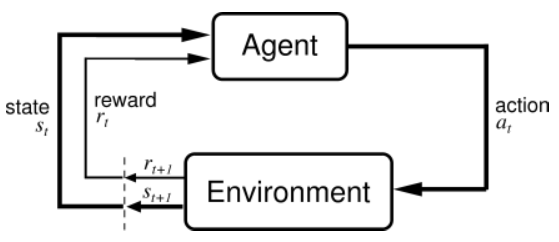
\includegraphics[scale=0.9]{agent-env-cycle.png}
\caption{The agent-environment cycle (Sutton and Barto, 1998).}
\vskip -0.2in
\label{fig:agent-env-cycle}
\end{figure}

The agent interacts with the environment with the help of three signals: a state signal, which describes the current state of the environment; an action signal, by which the agent interacts with the environment and a scalar reward signal, a feedback from the environment on the desirability of the immediate consequences of the action. At each time step of the agent-environment cycle, the agent senses the current state of the environment and applies an action. This action causes the environment to transition into a new state. After each state transition a reward (possibly zero) is passed to the agent. This reward evaluates the quality of the taken action. Along with the reward the agent senses the new environmental state. This process happens at each time step. The agent does not control state transitions and reward received. Instead the transition function and a reward function along with the set of possible actions and the set of all possible states belong to the environment which is often assumed to be a Markov decision process (MDP) (Bertsekas, 1995\nocite{bertsekas1995dynamic}). \\

Mathematically speaking a MDP consists of 2 sets and 2 functions. The two sets are the set of all possible states $\textit{S}$ and a set of all possible actions $\textit{A}$. The two functions are the transition function $\emph{f}$ and the reward function $\rho$. During interaction between the agent and the environment transition function $\emph{f}$ changes the state of the environment in response to the action signal. Right after state transition the reward function $\rho$ produces a scalar reward signal, i.e. immediate reward for an agent. During a time step $\emph{t}$ the agent applies action $\emph{$a_{t}$}$ in the state $\emph{$s_{t}$}$. The state changes to $\emph{$s_{t+1}$}$ according to the transition function $ f : S \times A \rightarrow S $:

$$\emph{$s_{t+1}$} = \emph{f}(\emph{$s_{t}$},\emph{$a_{t}$})$$

And the agent receives the scalar reward $\emph{$r_{t+1}$}$, according to the reward function $\rho$ : $\emph{S}$ $\times$ $\emph{A}$ $\rightarrow$ $\mathbb{R}$:

$$\emph{$r_{t+1}$} = \rho(\emph{$s_{t}$},\emph{$a_{t}$})$$

It is important to notice that both functions $f$ and $\rho$ can be either deterministic or stochastic.

The agent chooses actions according to its policy. The policy manifests which actions to pick at particular states $\pi$ : $\emph{S}$ $\rightarrow$ $\emph{A}$ :

$$\emph{$a_{t}$} = \pi(\emph{$s_{t}$})$$

Because environment is represented as a Markov decision process, it has the Markov property. That is given only $\rho$, $\emph{f}$, $\emph{$a_{t}$}$, $\emph{$s_{t}$}$ it is possible to determine the probability distributions of $\emph{$s_{t+1}$}$ and $\emph{$r_{t+1}$}$. This implies that all of the information required to make optimal decisions is contained within the current state vector $s_{t}$ - the agent need not take into account any historical information about previous states and actions. A good example is the chess game. One doesn't need to know the previous moves to decide the current move. It is enough to know the current positions of all figures on a board to make a decision.


\subsection{Agent's goals.}
On every stage of the decision process an agent chooses an action. The quality of the chosen action is evaluated and a reward is returned to the agent. This setting allows us to formalize the goal of the agent. The goal of the agent is an optimization problem of maximizing the amount of rewards throughout a course of interaction between agent and envrionment . In other words the agent must decide which sequence of actions will result in maximum of the rewards.

This formalization of the goal naturally reflects the learning process found in people and animals and thus allows to model many of the problems found in real life.

A \textit{return} is a cumulative sum of rewards obtained by the agent starting at some state $s_{0}$
$$\gamma^{0}\textit{r}_{1}+\gamma^{1}\textit{r}_{2}+\gamma^{2}\textit{r}_{3}+...$$

Here, the discount factor $\gamma$ $\in$ [0,1). First, this $\gamma$ guarantees convergence over the infinite horizon and second it denotes that the agent gives more weight to immediate rewards rather than delayed rewards.

Alternatively the return could be written like this:

$$ \emph{$R^{\pi}$}(s_{0}) = \sum_{t=0}^{\infty}\emph{$\gamma^{t}r_{t+1}$} = \sum_{t=0}^{\infty}\emph{$\gamma^{t}\rho$}(\emph{$s_{t}$},\emph{$\pi$}(\emph{$s_{t}$})). $$

And again $\gamma$ is the discount factor and $\emph{$s_{t+1}$}$ = $\emph{f}$ ($\emph{$s_{t}$}$,$\emph{$\pi$}$($\emph{$s_{t}$}$)) for $\emph{t}$ $\geq$ 0 and $\emph{$\pi$}$ is the policy being used.

Essentially, $ \gamma $ converts an infinite horizon MDP into a finite one. It is important to notice that in some cases it is possible to remove $ \gamma $ completely. For example, consider a case of a finite MDP with a -1 penalty for each move of an agent. In this setting this penalty will essentially work as $\gamma$.

\subsection{Dynamic Programming influence.}

Dynamic programming (Bellman, 1956\nocite{bellman1956dynamic}) is the scientific discipline centered around calculating the optimal policies for a given MDP. It has a strong assumption that we have a perfect model of the MDP (full knowledge of the transition and the reward functions).

Reinforcement learning has a strong connection to the dynamic programming. As was said before the dynamic programming requires the knowledge of both transition and reward functions. But in some scenarios this information is not available to us. Cases like these are the natural application of the reinforcement learning. The following paragraphs will describe terms that are common to both the dynamic programming and the reinforcement learning.

\subsubsection{Value Functions and Bellman Equation.}

A large optimization problem of maximizing a reward over all stages can be broken into a sequence of smaller problems. Each of these small problems is centered around picking an action which will maximize the combination of the immediate reward and a cumulative sum of rewards that follows the next state of the environment. This requires us to have some means to store and access the cumulative reward associated with each state of an environment.

A \textit{Value function} is a function that takes a state (or a combination of a state and an action) and returns the expected future reward that follows that state (or state-action). In essence, a value function describes the "goodness" or value of visiting a state and allows the agent to compare states with each other.

The value of a state $s_{t}$, at time step $t$, depends on the rewards $ r_{t+1},r_{t+2},... $. Which in turn depend on actions being taken at time steps $ t, t+1,... $. Actions of course depend on a policy being used by a decision-maker. Thus a value function of a state $s$ is denoted $V^{\pi}(s)$, with regard to some policy $\pi$, which underlies a decision making process.

Formally we can write
$$ V^{\pi}(s)=E_{\pi}\{R_{t}\;|\;s_{t}=s\} = E_{\pi}\left\{\displaystyle\sum_{k=0}^{\infty}\gamma^{k}r_{t+k+1}\;|\;s_{t}=s\right\}. $$

Function $V^{\pi}$ is called the \textit{state-value function} for policy $\pi$. The state-value functions are good for conveying the theory of multi-step decision processes. In practice, however, they are replaced by so called \textit{action-value functions}. The action-value function estimates the value of not only visiting a state $s$ but also of taking some action $a$ at that state, and subsequently following a policy $ \pi $. Formally we can write
$$ Q^{\pi}(s,a)=E_{\pi}\{R_{t}\;|\;s_{t}=s,a_{t}=a\} = E_{\pi}\left\{\displaystyle\sum_{k=0}^{\infty}\gamma^{k}r_{t+k+1}\;|\;s_{t}=s,a_{t}=a\right\}. $$

We can further notice that
$$ V^{\pi}(s)=E_{\pi}\{R_{t}\;|\;s_{t}=s\} $$
$$ =E_{\pi}\left\{\displaystyle\sum_{k=0}^{\infty}\gamma^{k}r_{t+k+1}\;|\;s_{t}=s\right\} $$
$$ =E_{\pi}\left\{r_{t+1}+\gamma\displaystyle\sum_{k=0}^{\infty}\gamma^{k}r_{t+k+2}\;|\;s_{t}=s\right\} $$
$$ =E_{\pi}\{r_{t+1} + \gamma V^{\pi}(s_{t+1})\;|\;s_{t}=s\}. $$

This equation is called the \textit{Bellman equation} for $ V^{\pi} $. The Bellman equation describes the connection between the value of a current state and the values of possible successor states. This fundamental recursive  relationship forms the foundation for a number of techniques to estimate correct values for $V^{\pi}$.

\subsubsection{Optimal Value Functions.}

Value functions allow us to compare different policies with each other, and naturally (because we are working with finite MDPs) there will be at least one best policy. To illustrate this we can visualize the given MDP as a tree. The tree's root is a starting state. Each branch of the tree represents a sequence of decisions (a policy) and the corresponding rewards. When the tree is finite there are a finite sequence of scalar rewards corresponding to each branch of the tree. One of those sequences will be the maximum. We can still apply the same logic even if the given MDP is infinite. In fact this is one of the reasons for using the discounting factor in the definition of return. The discounting factor allows us to represent the infinite MDP as the finite tree of decisions. We define a policy $\pi$ to be better than a policy $\pi'$ if it achieves higher or equal expected return for all states $s \in S $. Designation for optimal policy is $ \pi^{*} $.

Any policy leads to a value function and naturally the optimal policy $ \pi^{*} $ leads to the optimal value function $ V^{*} $. Formally we define $ V^{*} $ as

$$ V^{*}(s) = \max_{\pi}V^{\pi}(s), \;\;\;\;\text{for all}\; s \in S. $$

Now we can reformulate the reinforcement learning problem as finding the optimal policy $ \pi^{*} $ and associated optimal value function $ V^{*} $.

\subsubsection{Value Iteration.}

We now turn to how estimate the optimal policy. One particular algorithm is called \textit{value iteration}. This is an iterative algorithm which starts with any randomly initialized value function $V_{0}$. With each iteration $k$, the algorithm produces an approximation $V_{k}$, until it converges to the optimal value function $V^{*}$.

The value function is updated according to the following update rule:

$$ V_{k+1}(s) = \max_{a}\displaystyle\sum_{s'}T(s,a,s')\;[R(s,a,s')+\gamma V_{k}(s')], \;\;\;\;\text{for all}\; s \in S, $$
where $ T(s,a,s') $ is the probability to transition to the state $s'$ given state $s$ and action $a$, and $ R(s,a,s') $ is the immediate reward for transition to the state $s'$ given state $s$ and action $a$.

Here index $k$ can be viewed as the number of future rewards ahead that we are taking into account. For example, $k=0$ means that we are considering 0 time steps ahead, meaning that we are not considering even immediate reward.

\subsubsection{Policy Iteration.}

One of the disadvantages of the value iteration algorithm is due to the stopping criteria of the algorithm. In order to find whether we should stop the algorithm we need to observe the values for iterations $k$ and $k+1$. We can stop the algorithm only when we have a significant evidence that the values for all states are no longer improving. This gives rise to the situation when the optimal action for each state is already identifiable but there is still some difference between $ V_{k} $ and $ V_{k+1} $, for example due to small learning rate. Thus the algorithm may spend unnecessary amount of time just to meet formal criteria of convergence.

The algorithm called \textit{policy iteration} (Bellman, 1956\nocite{bellman1956dynamic}) is able to address this particular problem. The first step of the policy iteration algorithm is called the \textit{policy evaluation} (Bellman, 1956\nocite{bellman1956dynamic}). During the policy evaluation step, the algorithm is given any intermediate policy $ \pi_{i} $. This policy is then evaluated using the following update rule:

$$ V_{k+1}^{\pi_{i}}(s) = \displaystyle\sum_{s'}T(s,\pi_{i}(s),s')\;[R(s,\pi_{i}(s),s')+\gamma V_{k}^{\pi_{i}}(s')], \;\;\;\;\text{for all}\; s \in S, $$
where $ T(s,\pi_{i}(s),s') $ is the probability of transition to the state $s'$ given state $s$ and action $ \pi_{i}(s) $, and $ R(s,\pi_{i}(s),s') $ is the immediate reward for transition to the state $s'$ given state $s$ and action $\pi_{i}(s)$.

The policy evaluation step has a lot of similarities with the value iteration algorithm. Only in the policy evaluation we are not looking for a maximum over all possible actions and we are using a fixed policy $ \pi_{i} $.

Once the policy evaluation has converged, we proceed to the \textit{policy improvement} (Bellman, 1956\nocite{bellman1956dynamic}) step. We update the intermediate policy $ \pi_{i} $ according to the following rule:
$$ \pi_{i+1}(s) = \arg\max_{a}\displaystyle\sum_{s'}T(s,a,s')\;[R(s,a,s')+\gamma V_{k}^{\pi_{i}}(s')], \;\;\;\;\text{for all}\; s \in S, $$
where $ T(s,a,s') $ is the probability to transition to the state $s'$ given state $s$ and action $a$, and $ R(s,a,s') $ is the immediate reward for transition to the state $s'$ given state $s$ and action $a$.

The stopping criteria for the policy iteration is reached when we no longer able to improve intermediate policy $ \pi_{i} $ and thus we declare $ \pi_{i} $ to be the optimal policy $\pi^{*}$.

The advantage of the policy iteration over the value iteration lies within the policy evaluation update rule. This update rule doesn't have the maximum over all action operator $(\max_{a})$, since the policy under evaluation is fixed; This gives a significant speed of convergence advantage.


\subsection{Q-Learning.}
\label{sec:q-learning}
Policy iteration does not directly translate to the realms of the reinforcement learning as it requires the knowledge of a model of an environment (knowledge of reward and transition functions). Look at the update rule for the policy evaluation:
$$ V_{k+1}^{\pi_{i}}(s) = \displaystyle\sum_{s'}T(s,\pi_{i}(s),s')\;[R(s,\pi_{i}(s),s')+\gamma V_{k}^{\pi_{i}}(s')]. $$
And the update rule for the policy improvement:
$$ \pi_{i+1}(s) = \arg\max_{a}\displaystyle\sum_{s'}T(s,a,s')\;[R(s,a,s')+\gamma V_{k}^{\pi_{i}}(s')]. $$
They both require the knowledge of the functions $T$ and $R$, where $T$ is a state-transition function and $R$ is a reward function.

Reinforcement learning equivalent of policy iteration is called \textit{Q-Learning} (Watkins, 1992\nocite{watkins1992q}). Q-Learning, like DP value iteration, makes sure that any randomly initialized Q function converges to optimal action-value function $Q^{*}$. See Algorithm~\ref{alg:q-learning} for details.
\begin{algorithm}[tb]
   \caption{Q-Learning}
   \label{alg:q-learning}
\begin{algorithmic}
   \STATE {\bfseries Input:} Initialize $Q(s,a)$ randomly
   \REPEAT
       \STATE Initialize starting state $s$
       \REPEAT
           \STATE Choose $a$ from $s$ using policy derived from $Q$
           \STATE Take action $a$, observe $r$, $s'$
           \STATE $Q(s,a) \leftarrow Q(s,a) + \alpha [r + \gamma\; max_{a'}Q(s',a') - Q(s,a)] $
           \STATE $ s \leftarrow s'$
       \UNTIL{$s$ is terminal}
   \UNTIL{no more episodes}
\end{algorithmic}
\end{algorithm}
Q-Learning is a temporal-difference learning algorithm (Sutton and Barto, 1990\nocite{Sutton90time-derivativemodels}). The value iteration algorithm uses an expected value operator which requires knowledge of the state-transition function. Temporal-difference learning algorithms work around this by modifying update rule to work with raw experience. The update rule is slightly modified but essentially it does the same job only without the expected value operator:

$$ Q(s_{t},a_{t}) \leftarrow Q(s_{t},a_{t}) + \alpha \; \left[\;r_{t+1} + \gamma\; \max_{a}Q(s_{t+1},a) - Q(s_{t},a_{t})\;\right]. $$

Q-Learning requires several criteria to be met:
\begin{itemize}
  \item Underlying problem must be a Markov Decision Process.
  \item Learning rate $ \alpha $ should decrease to zero.
  \item Every state-action pair should be tried infinitely many times.
\end{itemize}
However, in practice the algorithm converges without some of these strict criteria. For example, in many cases the algorithm is able to converge with fixed $ \alpha $ parameter.

\subsection{Off-policy and On-policy algorithms.}
Previous section noted that temporal-difference methods such as the Q-Learning must be built in a way that ensures that every state-action pair is visited infinitely many times. This criterium is essential from the convergence point of view, remember that in the reinforcement learning a reward function is unknown for a learning algorithm and the only way to find the optimum sequence of actions is to try them all and calculate which one produces higher return. This means that the learning algorithm must at some point ignore a greedy action suggested by his current approximation of an optimal value function and instead choose some other action hoping that it will lead to a higher return.

One can run a series of episodes starting from the same starting state and record the return in each of the episodes. The average of those returns may differ from the value of the starting state predicted by the learned optimal Q-function. That is there will be a difference between the learned optimal Q-function and the actual results while the agent is learning. This behaviour is due to:
\begin{itemize}
  \item Q-learning learns the value of optimal sequence of actions given any starting state.
  \item The algorithm will introduce a randomness into action-selection process to insure that every state-action pair is selected (required by proof of convergence). Thus the actual sequence of actions taken by the agent will almost never be optimal.
\end{itemize}

Off-policy algorithms, such as Q-learning, do not record the actual value of each state-action pair, rather they record optimal value; They miss the fact that during each action-selection phase there might be a random action with potential negative outcome. As a result the agent might easily identify the greediest action among available actions but it will miss the fact that taking that greedy action might potentially result in big penalties due to possible exploratory actions.

On the other hand, on-policy methods do take into account the randomness associated with the action selection mechanism of the policy being followed. Thus the values $ Q_{\pi}(s,a) $, for each state action pair, reflect the average of all sequences of actions that are possible under the policy $ \pi $.

Q-learning is ideal for applications where an identification of optimal policy is the only goal. That is when there is no harm done to the agent itself or other involved parties if the agent has performed an action which results in big penalties. An example is escaping from a maze - the goal is to find an optimal escape route. It doesn't matter how many times the agent was circling around the maze while exploring. On the other hand, if a Mars rover is exploring the surface of the planet, it becomes very expensive and potentially dangerous for the equipment.



\subsection{SARSA.}

Sarsa is a temporal-difference algorithm similar to Q-learning, except it is an on-policy method. Both algorithms are very similar; The only difference is the update rule employed in each of the algorithms. The Q-learning has the following update rule:

$$ Q(s,a) \leftarrow Q(s,a) + \alpha [r + \gamma\; max_{a'}Q(s',a') - Q(s,a)]. $$

Here the construct $ max_{a'}Q(s',a') $ reflects the fact that only the greediest path from successor state $ s' $ is taken into account while updating the state-action pair $ Q(s,a) $.

The Sarsa algorithm has the following update rule:
$$ Q(s,a) \leftarrow Q(s,a) + \alpha [r + \gamma\; Q(s',a') - Q(s,a)]. $$

Sarsa doesn't try to maximize the value with which to update $ Q(s,a) $. Instead,  $ Q(s',a') $ is the return from successor state after taking action $ a' $, which was selected according to the policy being followed by the agent.

\section{Multi-objective Optimization.}

Multi-objective reinforcement learning methods are built upon methods from general multi-objective optimization. Therefore this section will briefly describe the main concepts and techniques that were borrowed from general multi-objective optimization.

\subsection{Multi-objective Problem.}

Let $A$ be a set of all possible actions. Given $n$ objective functions $ f_{1}(),...,f_{n}() $ , we map each action $a$ from the set $A$ to a point $ (f_{1}(a),...,f_{n}(a)) $ in the $n-$dimensional objective space.

Multi-objective problem is the problem of finding actions $a$ from the set $A$ such that we are most satisfied with the reward vectors $ (f_{1}(a),...,f_{n}(a)) $.

\subsection{Tradeoffs.}

Multi-objective optimization aims to solve difficult real life problems and many of these problems involve objectives that conflict with each other. Introduction of these conflicting objectives means that in many cases we will not have a single best option. Or in other words we cannot improve all objective functions at the same time. Rather we will need to compromise between two or more objectives, gaining more value on one objective at the expense of the other(s).

\subsection{Dominance.}
\label{sec:dominance}
Given two solutions $a'$ and $a''$ we can map them into two points in the $n$-dimensional objective space:
$$ x'=(x'_{1},...,x'_{n}) \;\;\;\;\text{and}\;\;\;\; x''=(x''_{1},...,x''_{n})$$
where
$$ x'_{i} = f_{i}(a') \;\;\;\;\text{and}\;\;\;\; x''_{i} = f_{i}(a'') \;\;\;\;\text{for}\;\;\;\; i = 1,...,n $$
The point $x'$ is said to Pareto dominate (Pareto, 1896\nocite{pareto1896cours}) point $x''$ when
$$ x'_{i} \geq x''_{i} \;\;\;\;\text{for all}\; i, $$
and
$$ x'_{i} > x''_{i} \;\;\;\;\text{for at least one}\; i.\footnote{For consistency with reinforcement learning discussion it will be assumed that the agent's objective is to maximize the objective functions, whereas in most multi-objective optimization literature the goal is to minimize the objectives. In fact, the two cases are fundamentally equivalent.} $$

Dominated points by definition will imply the existence of solutions that achieve more on each of the objectives and because our goal is to maximize the objective function we may omit dominated solutions. On the other hand, we may find two solutions which outperform each other on one of the objectives. In this case we really cannot say which solution is better, since each of them excels on one of the objectives. We call them non-comparable solutions. The set of all non-comparable solutions constitutes the Pareto front (Pareto, 1896\nocite{pareto1896cours}).

\subsection{The Pareto Front.}

Every action $a$ in the actions space $A$ is getting mapped to a point $ (f_{1}(a),...,f_{n}(a)) $. The image of the set $A$ in the $n$-dimensional objective space is called $the\; range \;set\; R$. The subset of $R$ which consists of non-dominated solutions is called $the\; Pareto\;front$, as shown in Figure~\ref{fig:paretoFront}.

Now we can reformulate multi-objective problem as the problem of locating any of the points belonging to the Pareto Front. Which point should it be? All of the points are not comparable to each other. If the tradeoff is a matter of a personal preferences then a personal opinion is required to make a decision.
\begin{figure}[ht]
\vskip 0.2in
\centering
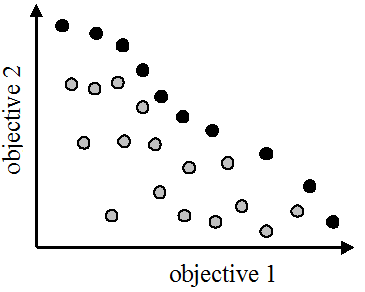
\includegraphics[scale=0.9]{paretofront.png}
\caption{The Pareto front is represented with black points. Each black point is a non-dominated solution. Grey points represent dominated solutions. Each gray point is dominated by at least one black point.}
\vskip -0.2in
\label{fig:paretoFront}
\end{figure}


\subsection{Selecting a Solution in The Pareto Front.}
\label{sec:Selecting-a-solution-in-the-Pareto-Front}
To reach a point in the Pareto front we need a scalar index which will reflect the preference between any two points. We can introduce a function $v$ defined on the $range \;set\; R$ with the following property:
$$ v(x_{1},..., x_{n}) \geq v(y_{1},..., y_{n}) $$
if and only if the point $ (x_{1},..., x_{n}) $ is more preferable or equal to the point $ (y_{1},..., y_{n}) $.

The following two sections will briefly describe two techniques to introduce that function $v$. These techniques are used in a large portion of multi-objective reinforcement learning algorithms and thus deserve a mention.

\subsubsection{Linear-Weighted Averages.}
Assume as before that the existence of a solution set $A$ and we also have $n$ objective functions $ f_{1}(),...,f_{n}() $. Each solution $ a\in A $ is mapped to a point $ (f_{1}(a),...,f_{n}(a)) $. Let
$$ \textbf{w} = (w_{1},...,w_{n}) $$
be a weight vector. Where
$$ w_{i} > 0, \;\text{for all }\; i $$
and
$$ \displaystyle\sum_{i=1}^{n} w_{i} = 1. $$

Let us pose an additional optimization problem: choose $a \in A$ that will maximize
$$ \displaystyle\sum_{i=1}^{n} w_{i}f_{i}(a). $$

Assume solution $a^{*}$ maximizes this given optimization problem. Let $ \textbf{x} = (f_{1}(a^{*}),...,f_{n}(a^{*})) $, in the $n$-dimensional objective space, with solution $a^{*}$.

The claim is that this point \textbf{x} must belong to the Pareto optimal set. If this point was not a member of the Pareto front there must another point \textbf{y} which dominates point \textbf{x}. But it cannot be since it would imply
$$ \displaystyle\sum_{i=1}^{n} w_{i}y_{i} > \displaystyle\sum_{i=1}^{n} w_{i}x_{i} $$
And we already know that point \textbf{x} is the maximum of the given optimization problem.

The more weight we apply to the specified objective the more favourable to the specified objective will be the identified point of the Pareto front. This allows us to perceive weights as a form of preference. However, setting the preferences a priori means human interaction and sometimes it is not so clear how to set these preferences.

Another limitation of this approach is the inability to locate concave points of the Pareto front. For example if the Pareto front has a concave shape then this approach will only locate extreme points.

\subsubsection{Lexicographical Ordering.}
Another widely used approach is to order objective functions $ f_{1}(),...,f_{n}() $ according to their importance.

Given two solutions $a^{1}$ and $a^{2}$ we say that $a^{1}$ is better than $a^{2}$ when $$ f_{i}(a^{1}) = f_{i}(a^{2}), \;\;\;\;\text{for}\;\;\;\; i = 1,...,n-1$$
and
$$ f_{n}(a^{1}) > f_{n}(a^{2}). $$

This approach is intuitively easy to understand and in fact in many problems it is possible to clearly differentiate which objective is more important.

\section{Multi-objective Reinforcement Learning Research.}

Reinforcement learning initially was applied to find optimal policies in single objective problems. However, in recent years there has been a significant increase in the interest towards multi-objective reinforcement learning. This can be explained by the fact that sometimes it is just impossible to express a sophisticated problem in terms of just a single objective, and naturally this gave rise to multi-objective reinforcement learning. For further motivation refer to Roijers et al. (2013)\nocite{roijers2013survey}.

This section will review the main work done on temporal-difference multi-objective reinforcement learning. It is only a review of the most seminal works, for more details please refer to Roijers et al. (2013)\nocite{roijers2013survey}. The first subsection will review temporal-difference methods based on the linear scalarization while the second subsection will consider non-linear methods. This separation is selected partially because linear methods are proven to converge while non-linear may not.

\subsection{Multi-Objective Markov Decission Processes (MOMDP).}
As was mentioned in Section \ref{sec:agent-and-environment}, in Markov decision processes the quality of taking action $a$ in a state $s$ is evaluated via immediate scalar reward signal $r$:
$$ r = \rho(s,a,s'), $$
where $s'$ is a successor state and $\rho()$ is a scalar reward function:
$$ \rho : S \times A \times  S \rightarrow \mathbb{R}. $$
In MOMDP there are $n$ such reward functions $\rho_{1},\rho_{2},...,\rho_{n}$ and the immediate reward signal is a vector: 
$$ \vec{r} = (\rho_{1}(s,a,s'),\rho_{2}(s,a,s'),...,\rho_{n}(s,a,s')). $$

Q-Learning, which was introduced in Section \ref{sec:q-learning}, was developed originally for single-objective MDPs, it can be seen from the update rule for this algorithm:
$$ Q(s_{t},a_{t}) \leftarrow Q(s_{t},a_{t}) + \alpha \; \left[\;r_{t+1} + \gamma\; \max_{a}Q(s_{t+1},a) - Q(s_{t},a_{t})\;\right]. $$
Here maximization operator assumes that there is a clear ordering between available options but in case of multi-objective MDPs there are options which are non-comparable to each other (see Section \ref{sec:dominance}). Hence some modification should be made to address this issue. 

\subsection{Linear Temporal Difference Learning.}

Before linear scalarization (see Section \ref{sec:Selecting-a-solution-in-the-Pareto-Front}) was used in reinforcement learning, Feinberg and Shwartz (1993)\nocite{Feinberg93constrainedmarkov} wrote an extensive paper on using linear scalarization in constrained Markov decision models. The authors proved the existence of optimal policies in such models and also proved that linear scalarization is able to identify members of the Pareto front. Even though this paper didn't mention reinforcement learning, it provided the necessary theoretical foundations for other researchers to try out linear scalarization in multi-objective reinforcement learning.

Karlsson (1997)\nocite{Karlsson97learningto}, in his PhD thesis, first tried to combine Q-learning algorithm and linear scalarization. The author argues that when dealing with multi-criteria problem, it is much better to break a complex state space into a number of smaller state spaces, so called modules. For each module we maintain a separate Q-function. It helps to avoid relearning when dealing with a complex task consisting of a number of independent sub-tasks.

Having multiple separate Q-functions, Karlsson faced a problem of how to administer the action selection process. He used the so called "greatest mass method". To determine a value of some action under this method, one needs to sum this action's Q-values across all modules. An action with the greatest overall sum is pronounced the greedy action. Essentially, this method is just a linear scalarization with all weights equal to one.

The author provided details of his test environment, which he called the simple driving domain (SDD). The SDD is a grid world with roads crossing it vertically and horizontally. The world is populated with different objects: street signs, traffic lights and obstacles. An agent controls a car. The agent has four goals: stay on a road, avoid obstacles, negotiate streetlights, follow street signs. All tasks are independent of each other. The author specifically created independent sub-tasks to test the modular approach.

The main point of Karlsson's research was to investigate how agents behave when the complex state space is decomposed into smaller sub-spaces. For this purpose he also created one agent which maintained a complex structure of the state space (monolithic approach). His results show that in many scenarios the modular approach performs as well as monolithic approach, while having a significant advantage in terms of speed of convergence.

Castelleti et al. (2002)\nocite{castelletti2002reinforcement} further explored linear scalarization. They were interested in applying reinforcement learning methods to a water reservoir management. As a case study they chose Lake Como, which is located in Northern Italy. This lake provides water supply to agricultural districts and hydroelectrical power plants.

It is possible to model this problem as an MOMDP. State information includes: current water level and information about natural water income. Actions govern how much water to release from the reservoir. In this paper the authors used two objectives: provide water and avoid flooding.

Unlike the work of (1997)\nocite{Karlsson97learningto}, the researchers didn't break the complex state space into smaller ones. However essentially their approach is the same - to identify greedy actions, one combines Q-values of each objective into a weighted sum. Only in this case, weighted sum is no longer uniform and weights could be arbitrary (as long as they sum to 1). They called their algorithm Qlp (Q-Learning planning). The authors approximated the Pareto front by having multiple independent tests - each test for one weight set.

In the experimental results section the authors compared their proposed approach with the results obtained with the help of stochastic dynamic programming approach (SDP); The QLP consistently outperformed the SDP.

It is important to notice that it was probably the earliest work where non-uniform weights were used.

Natarajan and Tadepalli (2005)\nocite{natarajan2005dynamic} used linear scalarization to sequentially learn multiple optimal policies. All the papers discussed so far
organized trials in similar manner:

\begin{enumerate}
  \item Set preferences for each objective.
  \item Initialize value function.
  \item Learn optimal policy for a the specified set of weights.
\end{enumerate}

All these steps need to be performed when preferences are changed. The authors noticed that the learnt value function for previous set of weights can be used to speed-up the learning process. If sets of weights are significantly different then one will not observe noticeable improvements. On the other hand, if the preferences correspond to nearby points in the objective space then the learning process will take full advantage of the value function learnt before. The authors propose mechanism which allows to determine which of the previously learnt policies should be used when the preferences are changed.

Two experimental domains are included in the paper: modified Buridan’s ass problem and network routing problem. The modified Buridan’s ass is the modification of the original problem (G{\'a}bor et al., 1998\nocite{gabor1998multi}). The modified version has an increased state-space - 3 by 3 grid world. A donkey is located in the middle of the grid world and two plates of food are located in top-left corner and bottom-right corner of the world respectively. The donkey must reach either of the plates with food to stay alive but every time he reaches for one of the plates the one might be stolen. Oveall there are three objectives: amount of food eaten, number of plates stolen and a number of moves made by the donkey. The authors demonstrate experimental results, which show a significant reduction of time-steps needed to learn optimal policies when prior value functions.

The network routing domain represents typical computer network with a number of nodes connected though a specified network topology. Three objectives are present: end to end delay, number of packets lost and power consumed by a node. Each state is represented by a current node and destination node. Actions are represented by neighbors of the current node through which the packet might be sent. Overall goal is to find an optimal routing policy according to specified preferences. The experimental results again demonstrate that learning from scratch for each set of weights takes a significantly loner amount of time than learning from prior policies.\\

\subsection{Non-linear Temporal Difference Learning.}

In many applications there is a natural ordering of the objectives; For example, consider a cleaning robot with two objectives: maintain a battery charged at all times, and clean an office. In this scenario there is natural ordering - the battery of the robot should never deplete (cleaning is not possible if the robot's battery is depleted), thus maintaining the battery level is considered more important. Non-linear temporal-difference methods can accurately reflect this ordering of the objectives and thus are more suitable for this domain.

More importantly, it has been shown (Yaman et al., 2010\nocite{Yaman20111290}) that people often employ lexicographic ordering of the objectives while making complex decisions.

One of the most earliest and most widely cited publications in MORL is Gabor, Kalmar and Szepesvari (1998)\nocite{gabor1998multi}. The publication first develops a solution for multi-criteria dynamic programming. After that the solution is modified to be extended to multi-criteria reinforcement learning.

The authors aimed at developing a mechanism to order policies. For this purposes, they used a minimum threshold on one of the objectives. This allowed authors to use only one objective as a maximization criteria. This paper builds upon lexicographical ordering of objective functions, which was described in the the multi-objective optimization section (Section 1.2.5).

After showing that this approach converges for abstract multi-criteria dynamic programming problem, the authors extend the technique for multi-criteria reinforcement learning.

This publication goes to a great extent describing mathematical proof of the proposed algorithm. Apart from mathematical aspects, the authors also included experimental results. Using a game of tic-tac-toe, the authors were able to show that their algorithm was able to identify optimal policy. They used two objectives: to win a game and to do it as fast as possible.

Van Moffaert et al. (2012)\nocite{van2012scalarized} proposed to use Chebyshev scalarization function. They used Chebyshev distance in the process of evaluating a set of actions. To successfully use this distance the authors introduced a so called utopian point $z^{*}$ in the objective space. After applying scalarization function to any state-action combination $(s,a)$ we obtain a scalarized Q-value (SQ):
$$ SQ(s,a) = \max_{o=1...m} w_{o} \cdot | Q(s,a,o) - z^{*}_{o} | $$
, where $m$ is the number of objectives. Given any state $s$ and all available actions $a$, we define a greedy action to be a solution to the following optimization problem:
$$ \min_{a} SQ(s,a). $$

The authors tested their approach on two well studied multi-objective reinforcement learning problems: the Deep Sea Treasure and the multi-objective Mountain Car. They were able to demonstrate that on both problems their non-linear scalarization approach was able to locate more optimal polices than usual linear scalarization.

Van Moffaert et al. (2013)\nocite{van2013hypervolume} proposed to use hypervolume indicator to guide action selection process. Their action-selection strategy (algorithm~\ref{alg:hb-as}) drastically differs from both linear and non-linear scalarization methods.

The agent maintains a list $l$ of points in the objective space. The list $l$ is empty at the beginning of an episode. On every step of the episode we map selected state-action to the objective space, according to q-value of the state-action pair. The resulting point is added to the list $l$.

Given any state $s$ and some available action $a$, the proposed strategy maps this action to a point in the objective space. After that we add this point to the list $l$ and calculate the hypervolume. The action is called greedy when it has the biggest contribution to the hypervolume.

The list $l$ is empty at the beginning of an episode. On every step of the episode we map selected state-action to the objective space, according to q-value of the state-action pair. The resulting point is added to the list $l$.

This approach utilizes search in the objective space of a problem. That is the main difference from the methods based on the scalarization, where we take q-values for each objective and transform it to a single value. However, this algorithm also uses Q-learning as underlying learning mechanism.

\begin{algorithm}[tb]
   \caption{Hypervolume based action-selection}
   \label{alg:hb-as}
\begin{algorithmic}
   \STATE {\bfseries Input:} a state $s$, list $l$ of Q-values
   \STATE  $volumes \leftarrow \{\} $
   \FOR{ $\text{each action}\;a\; \text{available at given state}\;s$ }
       \STATE  $ \text{create m-component vector}\; \textbf{r} $
       \FOR{ $ \text{i = 0 to m} $ }
       \STATE  $ r_{i} \leftarrow Q(s,a)\; \text{ for objective}\;i  $
       \ENDFOR
       \STATE $ hv \leftarrow \textit{getHypverVolume( l} + \textbf{r} \textit{)} $  \STATE add $hv$ to $volumes$
   \ENDFOR
   \STATE \textbf{return} $ \argmax_{a}\; volumes $
\end{algorithmic}
\end{algorithm}

The authors used the same set of test problems as in their work with Chebyshev scalarization function. On the Deep Sea Treasure problem, the hypervolume-based algorithm slightly outperformed one based on Chebyshev scalariation function, and significantly overpowered linear scalarization. On the multi-objective Mountain Car problem, the new algorithm performed comparably to Chebyshev scalarization function, and significantly outperformed one based on linear scalarization.

We know from Roijers et al. (2009)\nocite{roijers2013survey} that TD methods using non-linear scalarization may fail to converge due to the non-additive structure of the returns. While the work discussed in this section reports successful results based on non-linear temporal-difference, it may be that this is due to the specific characteristics of the small number of test problems on which performance has been evaluated. A need exists for more comprehensive evaluation of such methods.

\subsection{Simultaneous Learning of More Than One Policy.}

The algorithms reviewed in previous two sections belong to the class of single-policy methods, in that each run of the algorithm finds a single Pareto optimal policy (Vamplew et al., 2011\nocite{vamplew2011empirical}). To find an approximated Pareto front it is required to run the algorithm multiple times with different parameter setting (one for each Pareto optimal policy) and then manually combine them. In contrast, multi-policy algorithms aim to identify an approximated Pareto front in single run. This section will examine most important research in this direction.

Barrett et al. (2008) \nocite{barrett2008learning} propose an idea which allows to learn all optimal policies at the same time. They exploit the fact that Pareto front is essentially a convex hull object, under the assumption that linear scalarization is used to identify optimal points. This allows us to use convex hull operations in multi-objective reinforcement learning realms.

Single objective problems are naturally suitable for the Q-Learning update rule
$$ Q(s_{t},a_{t}) \leftarrow Q(s_{t},a_{t}) + \alpha \; \left[\;r_{t+1} + \gamma\; \max_{a}Q(s_{t+1},a) - Q(s_{t},a_{t})\;\right]. $$
Here we are backing a Q-value for previous state-action pair with immediate reward and maximum expected reward from successor state. In single-objective problems, it is always easy to find which sequence of actions will gain more rewards. So it always clear which value to use in this update rule. In contrast, multi-objective problems lack this clarity of choice. Now, we may have a multiple number of incomparable sequences of actions. The authors propose that we should use all optimal sequences of actions from a successor state and use all of them to back previous state-action pair. We no longer keep a single value for any state-action pair, rather we keep a set of values (convex hull of optimal Q-values). Thus we keep track of all possibilities for each state-action pair. At any time we can apply preferences (represented as a set of weights) to identify optimal policy.

The paper contains proof of correctness of this approach. The authors also included one test problem called Resource Gathering. This problem is a two dimensional grid world, an agent can locate two types of resources in this grid world. The agent receives a reward for each item brought home. However there are also two enemy positions were the agent can be attacked. If attacked, the agent receives a penalty and is moved to the home state.

This paper proposes an idea of learning optimal policies without ever specifying our preferences. This is a complectly opposite approach to most of the research done. Usually, we first set preferences and only after that we learn policy optimal to those preferences.

Lizotte et al. (2010) \nocite{lizotte2010efficient} also propose a mechanism to learn all optimal policies. They work with data from randomized medical treatments. These are the trials set up to find out how different patients react to different sequences of trials. The set of available actions consists of all possible treatments and set of all states consists of patient's health observations. They concentrate on two-objectives scenario, however, they do propose suggestions on how to extend their approach to more than two objectives. The first objective is the severity of the symptoms and the second objective measures the severity of the side-effects. \\

They use model-based approach; Originally state-transition probabilities and reward function are not known for apparent reasons but it is possible to analyze data from the trials and make approximations for both state-transition probabilities and reward function. Each episode:
$$ s_{0},a_{0},r_{0},s_{1},a_{1s},r_{1}, ... , s_{T},a_{T},r_{T} $$
is a history of prescribed treatments for one particular patient. At each time step $t$, $s_{t}$ is the health observations and $a_{t}$ is the prescribed treatment at this time step. These trajectories are used to make a model of the MDP. \\

After the the state-transition probabilities and the reward function are approximated, the authors use bottom-up dynamic programming approach. First they calculate the Q-function for the last time step $T$:
$$ Q_{T}(s,a,\delta) = r_{T}(s,a,\delta), $$
where $r(s,a,\delta)$ is
$$ r(s,a,\delta) = (1 - \delta) \cdot r_{0}(s,a) + \delta \cdot r_{1}(s,a), $$
where $ \delta \in [0,1] $, $ r_{0}(s,a) $ returns immediate reward for the first objective and $ r_{1}(s,a) $ returns immediate reward for the second objective. \\

After calculation of $ Q_{T} $ it is possible to calculate the Q-function for a time step $ t $ that precedes time step $ T $:
$$ Q_{t}(s,a,\delta) = r_{t}(s,a,\delta) + E_{s'|s,a} \left[\; V_{t+1}(s',\delta)\;\right], $$
where $ V(s,\delta) = \max_a Q(s,a,\delta). $

Modifying delta essentially changes preferences between the objectives and allows us to target different individual points of the Pareto front. The authors noticed that it is possible to choose a few values of $ \delta $ and calculate their respective representations in the objective space. After that it is possible to use linear spline interpolation to approximate all other points.

The authors compare their approach to the Barrett et al. (2008)\nocite{barrett2008learning} and show that asymptotically their approach is better in terms of time and space complexity.



























%\chapter{Empirical Evaluation}

\section{Introduction.}

Elaborate of absence of common means to empirically test algorithms from different authors in the field and how it complicates comparison of algorithms.

\section{Pareto dominance.}

Describe the idea of the Pareto front and Pareto dominance.

\section{Performance Metrics.}

Describe hypervolume metric.

\section{Methodology.}

Describe how are we going to use hypervolume metric to identify which of the algorithms performed better. 

\section{RL-Glue.}

Describe the RL-Glue.

\section{Benchmarks.}

Describe all present benchmarks.
\chapter{Empirical Evaluation.}

\section{Introduction.}

Whiteson and Littman (2011)\nocite{whiteson2011introduction} argued the importance of the empirical evaluation of reinforcement learning algorithms due to the natural limitations of other means to assess algorithms:

\begin{itemize}
  \item Subjective assessment (intuitive understanding) of an algorithm is prone to initial erroneous assumptions.
  \item Theoretical assessment (rigorous proof) often results in the mismatch of actual performance in a realistic domain with predicted theoretical performance. This is due to the fact that in realistic domains assumptions (that were used during rigorous proof) do not always hold.
\end{itemize}
Thus the empirical evaluation is an important part of a research process.

To conduct an empirical study one needs means to compare different algorithms. For example, classification algorithms are tested on data sets from special repositories. These data sets guarantee that different algorithms will be tested on the same set of benchmarks and thus they introduce more consistency into an assessment. They also allow an experimenter to make cross-comparison between different algorithms.

Reinforcement learning in general and multi-objective reinforcement learning in particular are very different from research areas like classification or clustering. Reinforcement learning is a multi-step decision making process with a number of actions available at each state at every time step. Add to this a factor of randomness associated with state transition and reward functions. Having all these factors substantially complicates the creation of a test problem. In reinforcement learning a test problem is not a static data set but rather a piece of software which reacts dynamically to the actions of an agent.

The absence of a central repository of test problems for multi-objective reinforcement learning lead to the fact that every published paper (prior to 2011\footnote{Vamplew et all. (2011)\nocite{vamplew2011empirical} introduced a number of test problems which were picked up later by other researchers.}) is disconnected from all other papers in terms of test problems. All papers described in the literature review present a brand new test environments. Moreover the majority of the papers use only a small amount of test problems, usually two\footnote{Peter, I still need some time to clarify how many test problems I will use, after that I will correct this section if needed}. This is in contrast with other areas of machine learning where each published paper is connected with other papers by using the same test data sets and the number of tested data sets is usually high, thereby allowing meaningful comparisons to be made between different algorithms.

The last section of the first chapter reviewed some of the most important research in temporal difference multi-objective reinforcement learning. All reviewed papers were mainly concerned with proving the convergence of their algorithms. In each paper authors presented a small number of their own test problems and their own methodology. It is enough in terms of convergence proof but clearly not enough to provide the full guidance about the types of problems for which the algorithm will perform well. Importantly, the convergence proofs do not generally provide any guarantees about the speed of convergence. The following information may be included in such a guidance:
\begin{itemize}
  \item Information about the structure of a reward function. An extrinsic reward function assigns zero rewards for the majority of state transitions of an environment except for special ones (for example, a transition to a goal state). In contrast, an intrinsic reward function is non-zero most of the time (for example, a time penalty applied at every time step to make an agent learn the shortest path). For more information about the application of both extrinsic and intrinsic reward functions in reinforcement learning refer to Uchibe and Doya (2007)\nocite{Uchibe2007}.
  \item Each test problem must be built around a particular property, which can be observed in realistic domains, such as a shape of the Pareto front.
  \item Each algorithm should be subjected to a range of different test problems with varying characteristics, to identify a realistic domain of application.
\end{itemize}

One can also notice the absence of a common methodology across all reviewed papers. Thus one cannot easily compare the results of an algorithm presented in one paper with the results of a different algorithm. Even if the same test problem is used, each methodology essentially incorporates a unique idea of how to show whether an algorithm is effective or not, and those ideas may drastically differ. Overall it substantially complicates the process of comparing the results presented in different papers. One major example can clarify the point. In multi-objective optimization the quality of an algorithm is evaluated by how close the algorithm approximates the Pareto front of a problem. Different methodologies measure this notion of "closeness" in a different way (Berry, 2008\nocite{berry2008phd}) and therefore it becomes meaningless to compare the results which were obtained using different methodologies.

The arguments above can explain the absence of empirical comparisons so far. No single attempt was made to perform a consolidated empirical evaluation of the proposed algorithms. Some of the papers provided empirical comparisons but only to prior versions of the same algorithms.

\section{The Empirical Evaluation Methodology.}

All of the works reviewed in the literature review chapter have the same limitations:
\begin{itemize}
  \item Limited number of test problems.
  \item No mention about the inability of the linear scalarization based algorithms to find concave points of the Pareto front. This limitation was quite known in traditional multi-objective optimization but until recently (Vamplew et al., 2008\nocite{vamplew2008limitations}) was never specifically mentioned in reinforcement learning theory. As a result later research work with uniform weights (Ferreira et al., 2012\nocite{F6363312}, Aissani, Beldjilali, and Trentesaux (2008)\nocite{aissani2008use}, Shabani (2009)\nocite{shabani2009incorporating}) also did not mention possible limitations of this approach.
  \item Each author or team of authors used their own evaluating methodology which complicates the cross-comparison.
\end{itemize}

This document will use the methodology previously proposed by Vamplew et al. (2011)\nocite{vamplew2011empirical}. This paper outlined very important aspects that should be introduced:
\begin{itemize}
  \item MORL algorithms should be tested on a wider range of test problems, and the properties of these problems should be understood to aid in interpreting the variations in the performance of algorithms.
  \item Standard benchmark problems and standard implementations of these problems should be established so as to facilitate comparison of the performance of different algorithms.
  \item Standard approaches to experimental methodology and reporting of results should be adopted, again to aid in the comparison of algorithms between papers. In particular numeric measures of performance will prove more useful for this purpose than the graphical reporting of results.
\end{itemize}

\subsection{Performance metrics.}
\label{sec:performance-metrics}
Every multi-objective problem implies the existence of a set of Pareto optimal solutions. The task of the learning algorithm is to find an approximation to that front. The quality of the approximation defines the quality of the algorithm.

Although every task has a true set of Pareto optimal solutions, machine learning algorithms can usually only approximate this set, and algorithms may vary in how well they estimate the front. Thus performance metrics should be introduced to facilitate in assessing the quality of the found set of Pareto optimal solutions.  Multi-objective reinforcement learning is similar to general multi-objective optimization in terms of a set of Pareto optimal solutions and so metrics previously considered in multi-objective optimization could easily be used in MORL.

Each approximation to a set of Pareto optimal solutions captures only particular points of the true set. How are these points spread relative to each other? How many points are captured? And to which extent does the the approximation cover the true set? All these important features could be encapsulated into a metric which allows us to compare two different learning algorithms. Early work in multi-objective optimization used scalar representations of these features. But each scalar metric captures only specific detail of the front such as diversity, cardinality or accuracy.

Later work in multi-objective optimization used different approach. Instead of multiple number of scalar metrics, composite metrics compatible with the notion of Pareto dominance were proposed. Berry (2008)\nocite{berry2008phd} presented arguments for composite metrics over a number of scalar ones. A number of such approaches were used in multi-objective optimization. For the purposes of this study, I will follow the lead of Vamplew et al. (2011)\nocite{vamplew2011empirical} and focus on the hypervolume metric.

\subsubsection{Hypervolume metric.}

The hypervolume metric (Zitzler and Thiele, 1999\nocite{zitzler1999pareto}) is a well-recommended composite metric which is used to evaluate the quality of an approximate Pareto front found by a learning algorithm. It measures the volume of the objective space region which is dominated by the points in the found Pareto front approximation. One additional point is also added before the volume is measured. This point is dominated by all points in the Pareto front approximation and serves as a reference point. An example is shown in figure~\ref{fig:hyperVolume}. It is important to note that the reference point must be consistent across different experiments because the value of the hypervolume is directly affected by the choice of the reference point. Even the same approximate Pareto front will give different values of hypervolume if different reference points are used, not to mention the ones produced by different algorithms. Thus it is safe to say that the choice of the reference point must be a part of the definition of the benchmark.

Given two learning algorithms, an experimenter can run them on the same test problem. Each algorithm will produce its approximate Pareto front. The experimenter can then calculate each approximation's hypervolume. The approximation which produces a higher value of the hypervolume is a better approximation to the true Pareto front. Importantly, improvements in any of the scalar measures of quality (diversity, cardinality and accuracy) will all be reflected in an increased value for hypervolume.

\begin{figure}[ht]
\centering
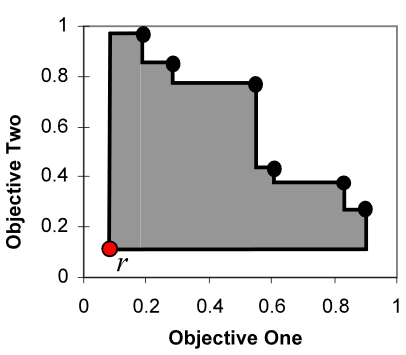
\includegraphics[scale=0.9]{hypervolume.png}
\caption{The figure shows how points from a Pareto front approximation and a reference point together define the region of objective space. The black dots are Pareto optimal solutions and the red dot is the reference point. The hypervolume of the enclosed region can be used as a measure of the quality of the frontal approximation.}
\label{fig:hyperVolume}
\end{figure}

\subsection{Experiment Structure.}
\label{sec:experiment-structure}
\subsubsection{Single-Policy Algorithms.}

Single-policy algorithms (Castelleti et al., 2002\nocite{castelletti2002reinforcement}, Gabor, Kalmar and Szepesvari, 1998\nocite{gabor1998multi}) are initialized with a set of preferences. After that the algorithm executes a number of learning episodes and hopefully it will learn the Q-function of the optimal policy for the specified preferences.

To illustrate the work of single policy algorithms consider the following example of a simple MDP which consists only of three time steps. On every time step two actions are available - left and right. State transition is deterministic i.e. each action always leads to the same successor state. For more details refer to Figure~\ref{fig:decisionTree}.\\

\begin{figure}[ht]
\centering
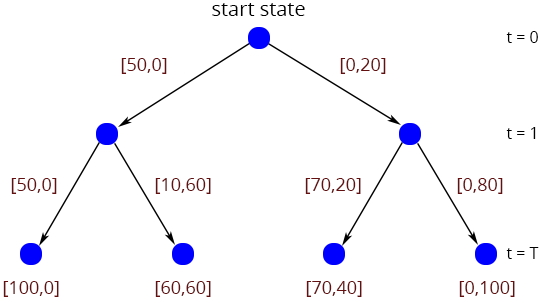
\includegraphics[scale=0.6]{decisionTree.png}
\caption{Blue circles represent states; Black arrows represent the actions. In every state left and right actions are available. State transition is deterministic and an action always leads to the same next state. Next to every arrow there is a vector of immediate rewards for choosing this action. The overall return starting from starting state is shown at the bottom of each branch.}
\label{fig:decisionTree}
\end{figure}

One can identify four different deterministic policies for this example MDP. Essentially, every branch of this tree defines a unique policy with it's associated return.

It is possible to look at this problem from a different perspective - in terms of the objective space. Figure~\ref{fig:exampleMDPFront} shows the two dimensional objective space for the example MDP problem. Each blue dot corresponds to a unique policy and it's coordinates are exactly this policy's return. Overall there are four points in the objective space, one for each policy. One can notice that this four points together constitute the Pareto front for this problem. This is because the example MDP problem doesn't have dominated policies.\\

\begin{figure}[ht]
\centering
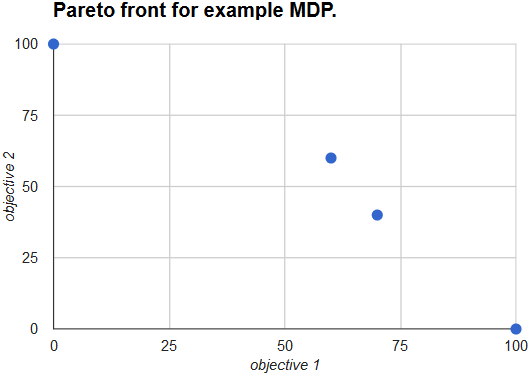
\includegraphics[scale=0.6]{exampleMDPFront.png}
\caption{Each blue dot is a unique policy from the example MDP problem. \textbf{NOTE:} Because the example MDP does not have dominated policies all four available policies together constitute the Pareto front for this problem.}
\label{fig:exampleMDPFront}
\end{figure}

Consider any single-policy algorithm, for example the linear scalarization approach discussed in Castelleti et al. (2002)\nocite{castelletti2002reinforcement}. This algorithm requires a set of weights to be specified before the algorithm can start learning; Let $ \textbf{w} = \{0.4,0.6\} $ be this set of weights. Essentially, this algorithm is the multi-objective reinforcement learning adaptation of the linear-weighted average algorithm from general multi-objective optimization. Linear-weighted average algorithm will find which of the available solutions (policies) will maximize the dot product of the return vector and the weight vector. In case of the example MDP, the policy with the return of [60,60] (see Figure~\ref{fig:exampleMDPOneMarkedPolicy}) will maximize the weighted average. The single-policy algorithm will learn the Q-function associated with this policy.

\begin{figure}[ht]
\centering
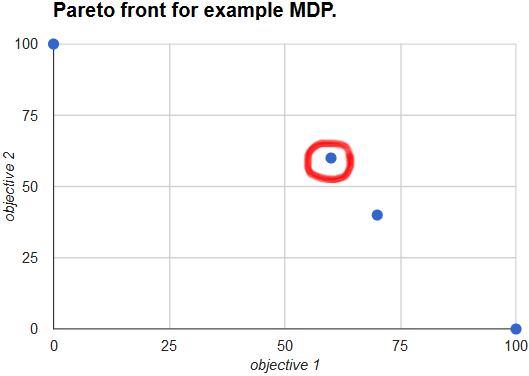
\includegraphics[scale=0.6]{exampleMDPOneMarkedPolicy.png}
\caption{The blue dot which represents the policy with return [60,60] is marked with a red circle. The linear-scalarized single policy algorithm mentioned above will learn the Q-function for the policy associated with the marked blue dot, when given weight \{0.4,0.6\}}
\label{fig:exampleMDPOneMarkedPolicy}
\end{figure}

Even though the algorithm was able to identify one element of the Pareto front, it is still preferable to find the whole approximation of the front as an algorithm is only useful if it performs well across it's entire range of parameters. The only way to achieve this with single policy algorithms is to reset the preferences every time the algorithm tries to identify another member of the Pareto front. This requires a special experiment design:

\begin{enumerate}
  \item Initialize an array of preferences, where each preference is an array itself (for example a set of weights).
  \item For each item in the array of preferences run a single-policy algorithm for a specified number of episodes. After the algorithm has converged, extract the greediest Q-value of a starting state and record it. \textbf{NOTE:} Notice that a priori an experimenter cannot identify which member of the Pareto front will be targeted by a certain set of preferences. One can only wait until the algorithm has learned the Q-function of a policy which is associated with the set of preferences. After that the greediest Q-value of the starting state will identify which point in the Pareto front was identified.
  \item Combine all recorded points into an approximation of the Pareto front.
\end{enumerate}

This experiment setting will allow us to create an effective approximation of the Pareto front of an underlying problem. It is vital to have this approximation if one is to compare the performances of different algorithms.

\subsubsection{Multi-Policy Algorithms.}
Single-policy algorithms are initialized with a set of parameters, usually its a set of weights - one for each objective. Eventually, this set of parameters gets mapped into one of the policies and the algorithm will learn the Q-function for this policy. As was mentioned before, an experimenter needs to prepare a number of sets of preferences (weights), and restart the experiment for every set of preferences, hopefully leading to a good approximation of the entire front.

However, it is possible to organize a learning process in a way which will allow us to learn more than one policy at a time. Instead of sequential working with each set of parameters one can work with all sets of parameters at the same time. For example, an algorithm might be given the following set - $ \{\;\{0.7,0.3\}, \{0.3,0.7\}\;\} $. Here the algorithm works with two sets of weights. Each set of weights represents the relative importance of each objective to an experimenter. Ideally, both sets will get mapped into different policies, although they both might get mapped into the same policy.  The algorithm then should learn the Q-functions for those mapped policies.

In this setting, one of the mapped policies is used as an active policy; It's Q-function is used during action-selection period. Other mapped policies are used only for learning purposes. This approach requires a special experiment design:
\begin{enumerate}
  \item Initialize an array of preferences, where each preference is an array itself(for example a set of weights).
  \item Create and initialize a number of Q-functions - one for each set of preferences.
  \item Run a specified number of episodes. In every episode, during every state-transition, use received immediate reward to update every Q-function.
  \item After learning is finished, run a greedy episode for each Q-function (if an environment's state-transition and reward functions are deterministic) or multiple episodes if the environment is stochastic in any way and record the resulting return.
  \item Combine all returns into an approximation of the Pareto front.
\end{enumerate}

However, not all multi-policy algorithms require such parameters (for example, Lizotte et al., 2010, Barrett et al., 2008). As was mentioned in Section \ref{sec:simultaneous-learning-of-more-than-one-policy}, these algorithms learn all optimal policies and use parameters only after a learning phase has finished.

There is a trade-off between two types of multi-policy algorithms:
\begin{itemize}
  \item Parallel learning of policies (each policy specified by a set of parameters) is easier to implement but it requires a somewhat complicated experiment design.
  \item On the other hand, learning all policies without using parameters requires a less complicated experiment structure but the algorithms themselves are much more complicated.
\end{itemize}
%Single-policy algorithms are initialized with a set of parameters, usually its a set of weights - one for each objective. Eventually, this set of parameters gets mapped into one of the policies and the algorithm will learn the Q-function for this policy. As was mentioned before, an experimenter needs to prepare a number of sets of preferences (weights), and hopefully those sets will approximate the Pareto front and restart the experiment for every set of preferences.
%
%This experiment setting is not very efficient - not only it takes more computer time but also significantly complicates an experiment design. Instead of sequential working with each set of parameters one can work with all sets of parameters at the same time. For example, an algorithm might be given the following set - $ \{\;\{0.7,0.3\}, \{0.3,0.7\}\;\} $. Here the algorithm works with two sets of weights. Each set of weights represents the relative importance of each objective to an experimenter. Ideally, both sets will get mapped into different policies, although they both might get mapped into the same policy.  The algorithm then should learn the Q-functions for those mapped policies.
%
%In this setting, one of the mapped policies is used as an active policy; It's Q-function is used during action-selection period. Other mapped policies are used only for learning purposes.
%
%Simultaneous learning of multiple policies is possible because state-transition dynamics provides enough information for more than one policy to be successfully updated. As an example consider state-transition depicted on Figure~\ref{fig:reasonForMPLearning}. Let $ \vec{w}^{1}=\{0.7,0.3\} $  and $ \vec{w}^{2}=\{0.3,0.7\} $ be two weight vectors. Each vector represents relative importance of each objective. Weight vectors $ \vec{w}^{1} $  and $ \vec{w}^{2} $ will get mapped into policies $ \pi^{\vec{w}^{1}} $  and $ \pi^{\vec{w}^{2}} $ respectively. Let both policies be deterministic.
%
%Further let $ \pi^{\vec{w}^{1}} $ be an active policy. At time step $ t $ action-selection was made according to active policy $ \pi^{\vec{w}_{1}} $ and let $ a_{t}=left $. Pair $ (s_{t}, a_{t}) $ makes an environment to transition to state $ s_{t+1} $ and the immediate reward [20,20] is received by a learning algorithm.
%
%\begin{figure}[ht]
%\centering
%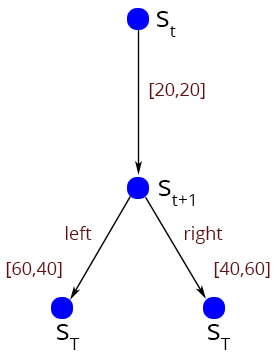
\includegraphics[scale=0.6]{reasonForMPLearning.png}
%\caption{An example state-transition. At time step $t$ the algorithm chose action $a_{t}\;=\;left$ according to the active policy $\pi^{\vec{w}^{1}}$. This resulted in transition to a state $s_{t+1}$ and immediate reward [20,20] was received by the algorithm. Even though policy $\pi^{\vec{w}^{2}}$ was not involved into action-selection it is still possible to update it's value of $Q(s_{t},a_{t})$.}
%\label{fig:reasonForMPLearning}
%\end{figure}
%
%At time step $ t+1 $ the algorithm needs to update $ Q(s_{t}, a_{t}) $ for both $ \pi^{\vec{w}_{1}} $  and $ \pi^{\vec{w}_{2}} $. To update $ Q(s_{t}, a_{t}) $ the algorithm needs to identify greedy action for a state $ s_{t+1} $ and use Q-value of that greedy action in combination with the immediate reward. For each policy the greedy action might be different but the immediate reward will be the same. This allows to update Q-function for the policy $ \pi^{\vec{w}^{2}} $ even though the state-transition was generated by the policy $ \pi^{\vec{w}^{1}} $.
%
%Table \ref{table:Qfunctionsfortplusone} shows the Q-functions for the state $ s_{t+1} $ for both policies $ \pi^{\vec{w}^{1}} $  and $ \pi^{\vec{w}^{2}} $. These two Q-functions are identical because both actions lead to the terminal state and only immediate reward is used during the update.
%
%{\renewcommand{\arraystretch}{1.2}
%\begin{table}[!htb]
%    \caption{\textbf{Left-hand side table} is the Q-function for the state $s_{t+1}$ for the policy $ \pi^{\vec{w}^{1}} $. \textbf{Right-hand side table} is the Q-function for the state $s_{t+1}$ for the policy $ \pi^{\vec{w}^{2}} $.}
%    \begin{minipage}{.5\linewidth}
%      \centering
%        \begin{tabular}{c|c|c}
%            state $\backslash$ action & left & right \\
%            \hline
%            $s_{t+1}$ & [60,40] & [40,60]
%        \end{tabular}
%    \end{minipage}%
%    \begin{minipage}{.5\linewidth}
%      \centering
%        \begin{tabular}{c|c|c}
%            state $\backslash$ action & left & right \\
%            \hline
%            $s_{t+1}$ & [60,40] & [40,60]
%        \end{tabular}
%    \end{minipage}
%    \label{table:Qfunctionsfortplusone}
%\end{table}
%
%For each policy $\pi$ the greedy action at time step $t+1$ is an action $a$ which will maximize the weighted sum:
%$$ \displaystyle\sum_{i=1}^{n} w^{\pi}_{i}Q^{\pi}_{i}(s_{t+1},a), $$
%where $n$ is the number of objectives. For the policy $ \pi^{\vec{w}^{1}} $ the weight vector is $ \vec{w}^{1}=\{0.7,0.3\} $ and the greedy action is $ left $ because
%$$ (60 \times 0.7) + (40 \times 0.3) > (40 \times 0.7) + (60 \times 0.3). $$
%Here $ (60 \times 0.7) + (40 \times 0.3) $ is the dot product $ \vec{w}^{1} \cdot Q^{\pi^{\vec{w}^{1}}}(s_{t+1},left) $ and $ (40 \times 0.7) + (60 \times 0.3) $ is the dot product $ \vec{w}^{1} \cdot Q^{\pi^{\vec{w}^{1}}}(s_{t+1},right) $. As you can see the dot product for action $left$ produces a higher value than the dot product for action $right$. The weight vector $\vec{w}^{1}$ has a higher value for the first objective. This will be translated into higher priority of the first objective and taking action $left$ in state $s_{t+1}$ results in higher expected return for the first objective. On the other hand for the policy $ \pi^{\vec{w}^{2}} $ the weight vector is $ \vec{w}^{2}=\{0.3,0.7\} $ and the greedy action is $ right $ because
%
%$$ (60 \times 0.3) + (40 \times 0.7) < (40 \times 0.3) + (60 \times 0.7). $$
%Here $ (60 \times 0.3) + (40 \times 0.7) $ is the dot product $ \vec{w}^{2} \cdot Q^{\pi^{\vec{w}^{2}}}(s_{t+1},left) $ and $ (40 \times 0.3) + (60 \times 0.7) $ is the dot product $ \vec{w}^{2} \cdot Q^{\pi^{\vec{w}^{2}}}(s_{t+1},right) $.
%
%Update rule for $ Q^{ \pi^{\vec{w}^{1}} }(s_{t},a_{t}) $ will take the following form:
%$$ Q^{ \pi^{\vec{w}^{1}} }(s_{t},a_{t}) \leftarrow Q^{ \pi^{\vec{w}^{1}} }(s_{t},a_{t}) + \alpha \; \left[\;r_{t+1} + \gamma\; Q^{ \pi^{\vec{w}^{1}} }(s_{t+1},left) - Q^{ \pi^{\vec{w}^{1}} }(s_{t},a_{t})\;\right]. $$
%And update rule for $ Q^{ \pi^{\vec{w}^{2}} }(s_{t},a_{t}) $ will take the following form:
%$$ Q^{ \pi^{\vec{w}^{2}} }(s_{t},a_{t}) \leftarrow Q^{ \pi^{\vec{w}^{2}} }(s_{t},a_{t}) + \alpha \; \left[\;r_{t+1} + \gamma\; Q^{ \pi^{\vec{w}^{2}} }(s_{t+1},right) - Q^{ \pi^{\vec{w}^{2}} }(s_{t},a_{t})\;\right]. $$
%Table \ref{table:updatedQfunctionsfortplusone} shows updated Q-functions for the state $s_{t}$ for both policies $\pi^{\vec{w}^{1}}$ and $\pi^{\vec{w}^{2}}$.
%
%{\renewcommand{\arraystretch}{1.2}
%\begin{table}[!htb]
%    \caption{\textbf{Left-hand side table} is the Q-function for the state $s_{t}$ for the policy $ \pi_{\vec{w}_{1}} $. \textbf{Right-hand side table} is the Q-function for the state $s_{t}$ for the policy $ \pi_{\vec{w}_{2}} $. Action $right$ was omitted from both Q-functions because it did not play any role in transition from state $s_{t}$ to state $s_{t+1}$.}
%    \begin{minipage}{.5\linewidth}
%      \centering
%        \begin{tabular}{c|c|c}
%            state $\backslash$ action & left & right \\
%            \hline
%            $s_{t}$ & [80,60] & ...
%        \end{tabular}
%    \end{minipage}%
%    \begin{minipage}{.5\linewidth}
%      \centering
%        \begin{tabular}{c|c|c}
%            state $\backslash$ action & left & right \\
%            \hline
%            $s_{t}$ & [60,80] & ...
%        \end{tabular}
%    \end{minipage}
%    \label{table:updatedQfunctionsfortplusone}
%\end{table}

\subsection{Benchmarking Software.}
As was mentioned before a test problem in reinforcement learning is a dynamic piece of software, which actively responds and changes according to the actions from an agent. The agent is also of a dynamic nature which in a similar manner dynamically reacts to the changes in the test problem. This is due to the inherent interactive nature of the the agent-environment cycle. For example every test problem should have the means (a function or a method) to accept an action from the agent. As well as means (again a function or a method) to pass information about state-transition and reward functions to the agent.

Even though test problems may have nothing in common in terms of realistic domains they represent, they still share those means of interaction with an agent or learning algorithm. Moreover in every problem the information that is passed between an agent and an environment is of very similar nature: the agent informs the environment about it's preferred action, the environment notifies the agent about the consequences of that particular action.

For a long time nobody took advantage of that fact; only different programming techniques were used to implement the interaction between the agent and the environment and also different programming languages and different platforms were used. Even if two authors used the same test problem it is possible that differences may exist in their implementations of that problem. This created a natural level of complexity which prevented the exchange of learning algorithms and test problems.

Eventually Tanner and White (2009)\nocite{tanner2009rl} created an open source software called RL-Glue. This software lays a foundation for empirical studies in reinforcement learning because it provides a necessary set of standards which allows researchers to connect the test problems with the learning algorithms from different researchers. The framework handles all the complexities hard work of connecting and passing information between algorithms and problems. For example, experimenters who want to test their newly developed algorithm on a set of well established test benchmarks does not need to think about how their code will interact with different problems; They just encapsulates the logic of their algorithm into standard functions. After that RL-Glue will be able to connect this algorithm to any test problem. Essentially, RL-Glue, by introducing a set of standard functions , allows researchers to plug-in agents, environments and experiments from different authors even created in different languages.

RL-Glue consists of three main modules as shown in Figure \ref{fig:rlglue}: an agent, an environment and an experiment. The agent is the module which encapsulates a learning algorithm. The environment is the module which encapsulates a particular test problem. The experiment module is a place where a researcher controls how many time steps per episode or how many episodes should be performed by the agent. All the interaction between the modules is handled by a central server RL-Glue server.

\begin{figure}[ht]
\vskip 0.2in
\centering
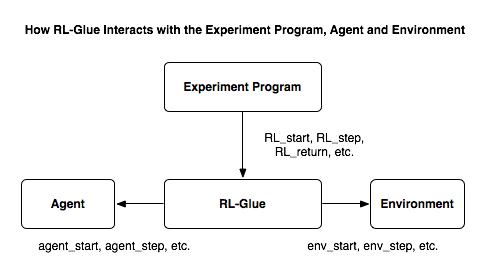
\includegraphics[scale=0.9]{glue.png}
\caption{This diagram depicts the interaction between all modules. As can be seen from the figure all modules are connected to a central RL-Glue server which in turn facilitate the exchange of information between all modules. Tanner and White (2009).}
\vskip -0.2in
\label{fig:rlglue}
\end{figure}
The plug-in nature of the RL-glue framework perfectly addresses three aspects of adequate methodology that were outlined before. Namely:
\begin{itemize}

\item The agent module encapsulates the learning algorithm. Each learning algorithm is a separate plug-in. Multiple numbers of learning algorithms can be attached to the RL-Glue simultaneously. This allows an experimenter to evaluate multiple algorithms simultaneously. A researcher just chooses which of the connected agents will be evaluated.

\item The environment module tackles aspect number two of the adequate methodology. Because the environment module is well-documented and well-standardized in terms of standard programming interfaces it allows the creation and reuse of standard test problems. This module eliminates connecting code needed previously. With plug-in architecture the researcher only needs to download a test problem and plug it into a running RL-Glue server without writing any code to connect the problem and the algorithm.

\item The experiment module tackles aspect number three of the adequate methodology. The experiment module is the plug-in where the researcher chooses the particular test problem and the particular learning algorithms that will be evaluated against that test problem. The experiment module is also a place where all the statistics are gathered and analyzed. This is achieved by introducing a standard message protocol between the agent module and the experiment module. Using this message protocol the agents can send information about learned Q-functions and policies to the experiment module. This is also a place where different performance metrics are applied. Each performance metric is created as a library with external functions which encapsulates the inner routines. Such performance metrics are stored separately in the library files and also could be accessible to the public. For example hypervolume performance metric will be introduced to RL-Glue as a part of this thesis and will be available publicly.

\end{itemize}

Originally, RL-Glue is a software for single objective reinforcement learning but it can be adapted to multi-objective (which is also a part of this thesis) by replacing scalar reward signal with a vector-valued signal.

\subsection{Multi-Objective RL-Glue framework.}
RL-Glue framework is a perfect testing platform for reinforcement learning but it is hardcoded to work with single-objective domains. As a part of the contribution made by this thesis the RL-Glue framework was extended to work with multi-objective domains. RL-Glue framework is an open source software which allowed me to thoroughly study the architecture of the framework and to introduce changes which allowed the RL-Glue framework to represent a reward signal as a vector.

\section{Benchmarks.}

Each benchmark or test problem is created to address a particular aspect of real-life problems. Thus a rich library of benchmarks should be available to adequately assess a learning algorithm. A suite of these benchmarks will allow to look at the learning from different point of views. Combined together, the benchmarks will allow researchers to evaluate how different algorithms cope with the following aspects of real-life problems:

\begin{itemize}

\item Multiple number of objectives. To test which algorithms cope better when the number of objectives is increased.

\item A range of benchmarks should be devoted to assess algorithms under stochasticity of reward and state transition functions.

\item One of the basic requirements is to create benchmarks with continuous state and action spaces.

\item Another important class of benchmarks is ones describing real-life problems with large dimensionality of state or action spaces that require the use of function approximation;

\item Problems with partially-observable states.

\item A mixture of episodic and continuing tasks;

\item Each real-life problem assumes existence of Pareto front of optimal solutions. This front exhibits a number of different characteristics. A number of benchmarks should be created to expose the learning algorithms to all possible characteristics of the Pareto front.

\item Characteristics of a reward structure, such as different combinations of intrinsic and extrinsic rewards.
\end{itemize}

Vamplew et al (2011)\nocite{vamplew2011empirical} already introduced a number of benchmarks with known Pareto fronts. This greatly facilitates in the evaluation of the multi-objectives algorithms. We will use this these benchmarks as the basis for the empirical studies reported in this thesis.

Some of the benchmarks presented in Vamplew et al (2011)\nocite{vamplew2011empirical} are already being widely adopted in the MORL community. For example, Van Moffaert et al. (2012)\nocite{vamplew2011empirical}, Brys (2013)\nocite{brysmulti} etc.

\subsection{Deep sea treasure.}
This test problem is a 10 by 11 grid world as shown in Figure \ref{fig:DSTOverview}. The grid represents an undersea surface with multiple number of treasure spots available. Each treasure spot has a different treasure value. The agent is represented as a submarine. Four actions are available to the agent - left, right, up, down. Each of the actions move the submarine by one square in appropriate direction; If an action results in the agent moving outside of the grid world then the agent is returned to his previous location. The reward signal for this problem is a two dimensional vector; the first component represents the amount of treasure that was found during a single episode, while the second component of the reward signal is an accumulated penalty over an episode (-1 for each move).

\begin{figure}[ht]
\vskip 0.2in
\centering
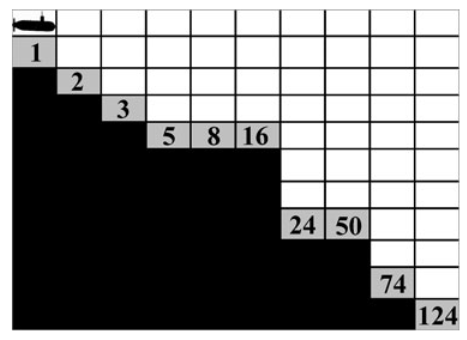
\includegraphics[scale=0.9]{dst.png}
\caption{Grid world for Deep Sea Treasure problem. Vamplew et al (2011).}
\label{fig:DSTOverview}
\end{figure}

The Deep Sea Treasure is an episodic test problem. Each episode the agent starts in the top-left corner of the gird world. During the exploration of the world the agent may find one of the treasure spots. Also, every time step the agent receives -1 penalty (to encourage shortest path learning); The episode finishes when the agent locates one of the treasures. After that the agent is returned to the starting state.

Also this test problem comes with a known Pareto front which is shown in Figure \ref{fig:DSTFront}. The form of the front is globally concave with number of local concavities.

\begin{figure}[ht]
\vskip 0.2in
\centering
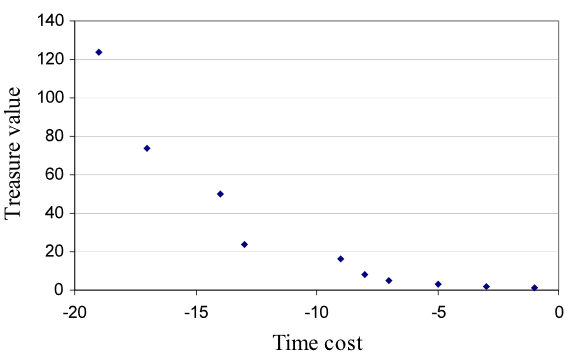
\includegraphics[scale=0.9]{dstPareto.png}
\caption{Pareto front for Deep Sea Treasure problem. Vamplew et al (2011).}
\label{fig:DSTFront}
\end{figure}

\subsection{MO-Puddleworld.}
This test problem is a two dimensional grid world with puddles located across the world as shown on Figure \ref{fig:PWOverview}. Each episode the agent starts at a random location and must reach the goal position(top-right corner) while avoiding the puddles. Four actions are available to the agent - left, right, up, down. In this test problem the reward signal is represented as a two dimensional vector; The first component is an accumulated time step penalty over an episode (-1 for each move), while the second component of the reward vector is an accumulated puddle penalty (each time the agent walks into a puddle a penalty is given to the agent).

\begin{figure}[ht]
\vskip 0.2in
\centering

\includegraphics[scale=0.9]{pw.png}
\caption{Grid world for the Puddleworld problem. Vamplew et al (2011).}
\label{fig:PWOverview}
\end{figure}

MO-Puddleworld is also an episodic problem. Each episode the agent starts in a random or fixed location and must find its way to the goal state; Once the agent reaches the goal state, the episode is finished and the agent is returned to the start state.

MO-Puddleworld is a modification of the original Puddleworld problem (Boyan and Moore, 1995\nocite{boyan1995generalization}). Although several modifications were introduced:

\begin{itemize}
  \item One composite reward signal of the original Puddleworld was broken into a two component vector as described above.
  \item Calculation of the puddle penalty is slightly changed - the 400 multiplication is omitted.
  \item Original problem had a noise movement which was added during every move of the agent. It was ommited in the MO-Puddleworld.
  \item The goal state in the original problem was a triangular shape but it was enlarged to a full 0.05 square in the MO-Puddleworld.
\end{itemize}

\subsection{MO-Mountain Car.}
This test problem represents a valley with a car that must escape from the valley. But the car's engine is too weak to overcome the gravity force so the car must first climb a hill on the left side of the valley with reverse acceleration to build enough momentum to escape from the valley through the hill on the right side. Three actions are available to the agent - full throttle forward, full throttle backward, and zero throttle. A penalty of -1 is received on all states except the goal state. There are two additional penalties: -1 for each reverse acceleration and -1 for each forward acceleration.

As well as the MO-Puddleworld, the MO-Mountain Car is also a modification of the original single objective problem (Sutton, 1996\nocite{sutton1996generalization}). The original problem was modified by extending the reward signal from a scalar representation to a three component vector as described above.

\subsection{Resource gathering.}
\label{sec:resource-gathering}
This test problem, originally proposed by Barrett and Narayanan (2008)\nocite{barrett2008learning}, represents a 2-dimensional grid world. Two types of resources are available for gathering - gold and gems. The goal of the agent is to gather resources (either one of them or both). Also there are locations where the hero can be attacked, the chance of being attacked is 10 percent, see Figure \ref{fig:RGOverview} for details. If the attack happens then the agent loses all gathered resources and receives a negative reward for the "enemy" objective; The agent is also returned to the base after the attack. Four actions are available to the agent - left, right, up, down. Each of the actions move the agent by one square in appropriate direction.

The reward signal is a 3-dimensional vector where the first component shows the penalty if the enemy attack has happened, the second component shows how much gold was collected during an episode and the third component shows how much gems were collected.

\begin{figure}[ht]
\vskip 0.2in
\centering
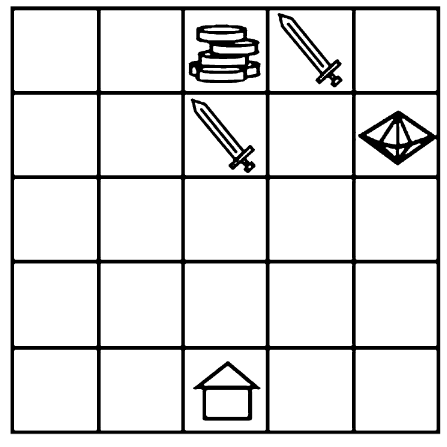
\includegraphics[scale=0.6]{rg.png}
\caption{Grid world for the Resource Gathering problem. Barrett and Narayanan (2008).}
\label{fig:RGOverview}
\end{figure}

Barrett and Narayanan (2008)\nocite{barrett2008learning} used Convex Hull Value Iteration algorithm and found six optimal policies as shown on Figure \ref{fig:RGAlloptimalPolicies}

\begin{figure}[ht]
\vskip 0.2in
\centering
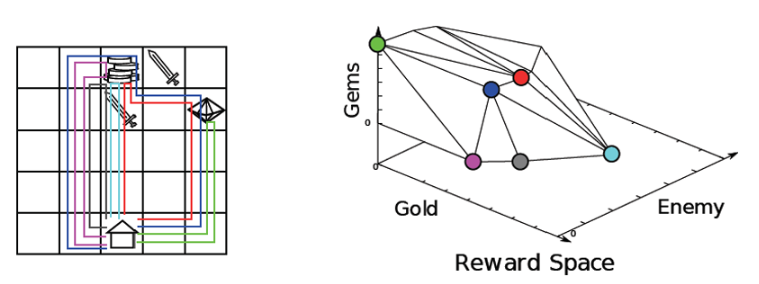
\includegraphics[scale=0.8]{rgpareto.png}
\caption{Optimal Policies for the Resource Gathering problem. The left hand side picture shows all non-dominated policies in the problem's state-space, while the right hand side shows the same policies in the objective space. Barrett and Narayanan (2008).}
\label{fig:RGAlloptimalPolicies}
\end{figure} 
\chapter{Evaluation of single policy multiobjective reinforcement learning algorithms.}

\section{Introduction.}
The last two chapters provided necessary background information, as well as arguments for empirical evaluation of multi-objective reinforcement learning algorithms. This and all following chapters will be concentrating on an empirical analysis of different groups of algorithms. This chapter will focus on single policy algorithms. That is, algorithms which upon completion will produce an optimal value function for one policy. Two of the most common approaches are based on the well-established techniques from the multiobjective optimization: linear-weighted averages and lexicographic ordering (see Section \ref{sec:Selecting-a-solution-in-the-Pareto-Front} for explanation of both techniques).

It is impossible to say which approach is better, rather like two non-dominated policies, as these techniques are not comparable. Both have strong and weak points and ultimately the decision on which algorithm to use should be based on a problem at hand. This chapter will present empirical results of both approaches for a range of test problems. Each of the problems exhibits a property found in realistic domains which will significantly affect the performance of an algorithm under consideration.

\subsection{Weighted Scalarization.}
Section \ref{sec:linear-temporal-difference-learning} documented how the linear-weighted averages algorithm was adopted in multi-objective reinforcement learning. Arguably the most seminal work in this direction was the linear-weighted average implementation by Castelleti et al., (2002\nocite{castelletti2002reinforcement}), which is essentially a weighted scalarization of objective functions to reduce a multi-objective problem to a single objective one.

Weighted scalarization allows an experimenter to locate a single point of the Pareto front. The located point depends on a set of weights which was given to the algorithm. By gradually changing the weights over objectives the algorithm can locate optimal value functions for different policies, thus approximating the Pareto front.

An experiment structure for this type of a single policy algorithm was given in Section \ref{sec:experiment-structure}. It is important to point out that a priori the experimenter does not know which weights correspond to which policy and the experimenter will need to perform a number of test learning episodes to get an idea of a shape of a Pareto front for some MOMDP.

\subsection{Thresholded Lexicographic Ordering.}
Gabor, Kalmar and Szepesvari (1998)\nocite{gabor1998multi} implemented lexicographic ordering of objectives in their algorithm$\footnote{Gabor et al did not provide a name for their algorithm. For care of reference, in this thesis we will adopt the Thresholded Lexicographic Ordering (TLO) name as used by Vamplewet al.}$ (see Section \ref{sec:non-linear-temporal-difference-learning}). Lexicographic ordering of objectives relies on restricting all but one of the objectives to a certain threshold values thus allowing to use a maximization operator on the last unrestricted objective. This requires domain knowledge which is not always practical to obtain, however, in many realistic domains it is possible to probe a problem with weighted scalarization to obtain a range of values for each of the objectives and use that knowledge to build a system of thresholds which will cover a Pareto front for the problem.
\begin{figure}[ht]
\centering
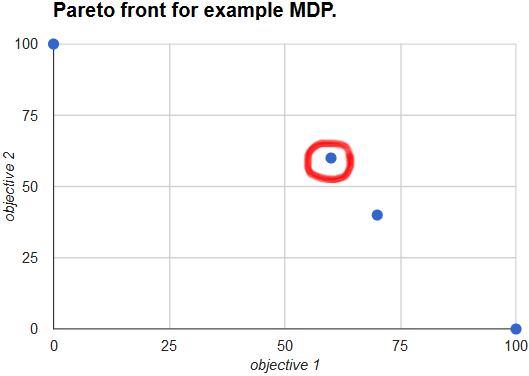
\includegraphics[scale=0.6]{exampleMDPOneMarkedPolicy.png}
\caption{Using the weighted scalarization will provide insights about points of a Pareto front for some problem. In this example the weighted scalarization identified one member of the Pareto front and obtained information can be used to specify thresholds for the thresholded lexicographic ordering algorithm. The blue dot which represents the policy with return [60,60] is marked with a red circle. The linear-scalarized single policy algorithm mentioned above will learn the Q-function for the policy associated with the marked blue dot, when given weight \{0.4,0.6\}}
\label{fig:how-tlo-works}
\end{figure}

To illustrate how weighted scalarization allows an experimenter to obtain the threshold values consider the Figure \ref{fig:how-tlo-works}. This is the example MOMDP with two objectives from Chapter two (see Section \ref{sec:experiment-structure}) with four non-dominated policies. An experimenter randomly chooses a set of weights $ \textbf{w} $ (for example let $ \textbf{w} = \{0.4,0.6\} $). This will make weighted scalarization to learn optimal value function for the policy with return [60,60] (marked with a red circle on the Figure \ref{fig:how-tlo-works}). After that the experimenter initializes the thresholded lexicographic ordering algorithm with the threshold of 60 for the first objective and starts the algorithm. The algorithm will try to maximize the second objective given that it satisfied the threshold for the first objective.

\section{Empirical Results.}

\subsection{Deep Sea Treasure.}
For problem specification see Section \ref{sec:deep-sea-treasure}.

Deep Sea Treasure is an interesting problem because of the fact that one of the objectives, treasure, is extrinsic and the second one, time, is intrinsic. In addition the Pareto front for this problem is globally concave. This structure of rewards is really suitable for showcasing advantages of TLO algorithm over WS.

Table \ref{tab:deep-sea-treasure} shows the results of WS and TLO runs on the Deep Sea Treasure. As was expected the WS algorithm was not able to find concave Pareto front members. Contrary to the WS, the TLO algorithm was able to locate concave Pareto front members. So the TLO was able to find extreme members of the Pareto front as well as intermediate, this leads to higher hypervolume values.

\begin{table}[t]
\centering
\def\arraystretch{1.5}
\begin{tabular}{|c|c|c|c|c|c|}
  \hline
  % after \\: \hline or \cline{col1-col2} \cline{col3-col4} ...
  & 10k & 20k & 30k & 40k & 50k \\
  \hline
  WS & 388 & 292 & 462 & 288 & 142 \\
  \hline
  TLO & 460 & 510 & 510 & 510 & 510 \\
  \hline
\end{tabular}
\caption{TLO and WS algorithms tested on Deap Sea Treasure. Reference point is (0,-20). Epsilon is 0.17, alpha is 0.9, gamma is 1.0. Step limit is 200 per episode.}
\label{tab:deep-sea-treasure}
\end{table}

\begin{figure}[ht]
\centering
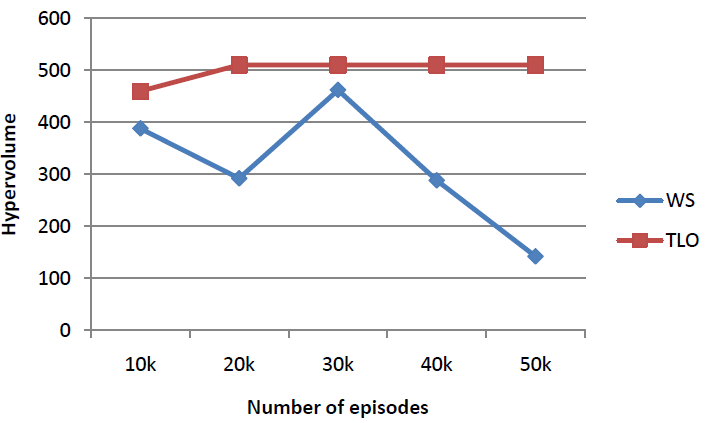
\includegraphics[scale=0.6]{DSTResults.png}
\caption{WS vs TLO tested on Deep Sea Treasure. Reference point is (0;-20). Epsilon is 0.17, alpha is 0.9, gamma is 1.0.}
\label{fig:ws-tlo-dst-results}
\end{figure}

\subsection{MO-PuddleWorld.}
For problem specification see Section \ref{sec:mo-puddleworld}.

The reward structure for MO-PuddleWorld has one intrinsic reward, namely the time penalty, which is -1 on all steps except goal state, when penalty is 0. The second reward, namely puddle penalty, is extrinsic. The MO-PuddleWorld test problem represents a state as a combination of two continuous variables: x position and y position. A 20 by 20 discretization was used in case of both the TLO and the WS algorithms. Tables \ref{tab:mo-puddleworld-1} and \ref{tab:mo-puddleworld-2} provide details of WS and TLO algorithms ran from 5 different starting positions. Fixed positions were used to remove the effects of noise due to random starting positions.

The results of the two algorithms are very similar. This can be explained by the nature of the problem itself. In the deep sea treasure problem the shape of the Pareto front provides a number of concave solutions and the TLO algorithm can converge to any point in that front, which increases the hypervolume. Contrary, the MO-PuddleWorld's Pareto front from most of the starting points is primarily convex in shape, and when concave solutions are available, a number of those solutions is very small and they contribute only slightly to the overall hypervolume attainable. So the TLO algorithm never receives a chance to showcase its benefits over the WS algorithm.

\begin{table}[t]
\centering
\def\arraystretch{1.5}
\begin{tabular}{|c|c|c|c|c|c|}
  \hline
  % after \\: \hline or \cline{col1-col2} \cline{col3-col4} ...
  & (0.25;0.6) & (0.35;0.55) & (0.3;0.55) & (0.3;0.7) & (0.2;0.7) \\
  \hline
  0 & 1084 & 988 & 99 & 99 & 99 \\
  \hline
  500 & 7998 & 8084 & 7984 & 8287 & 8087 \\
  \hline
  1000 & 7998 & 8084 & 7998 & 8297 & 8098 \\
  \hline
\end{tabular}
\caption{WS algorithm tested on MO-PuddleWorld problem with 5 different starting positions. Reference point is (-100,-100). Epsion is 0.15, alpha is 0.9, gamma is 1.0. Step limit is 100 steps per episode.}
\label{tab:mo-puddleworld-1}
\end{table}

\begin{table}[t]
\centering
\def\arraystretch{1.5}
\begin{tabular}{|c|c|c|c|c|c|}
  \hline
  % after \\: \hline or \cline{col1-col2} \cline{col3-col4} ...
  & (0.25;0.6) & (0.35;0.55) & (0.3;0.55) & (0.3;0.7) & (0.2;0.7) \\
  \hline
  0 & 99 & 100 & 99 & 99 & 99 \\
  \hline
  500 & 7984 & 8083 & 7984 & 8287 & 8087 \\
  \hline
  1000 & 7984 & 8083 & 7984 & 8287 & 8087 \\
  \hline
\end{tabular}
\caption{TLO algorithm tested on MO-PuddleWorld problem with 5 different starting positions. Reference point is (-100,-100). Epsion is 0.15, alpha is 0.9, gamma is 1.0. Step limit is 100 steps per episode.}
\label{tab:mo-puddleworld-2}
\end{table}

\subsection{MO-MountainCar.}
For problem specification see Section \ref{sec:mo-mountain-car}.

The reward structure for mountain car problem consists of 3 intrinsic rewards. The first is a penalty of -1 applied each time step, the second is a penalty of -1 applied at every backward acceleration and the third one is a penalty of -1 applied at every forward acceleration. The MO-MountainCar test problem represents a state as a combination of two continuous variables: a position and a velocity. A 170(position) by 140(velocity) discretization was used in case of both the TLO and the WS algorithms.

\begin{table}[t]
\centering
\def\arraystretch{1.5}
\begin{tabular}{|c|c|c|c|c|c|}
  \hline
  % after \\: \hline or \cline{col1-col2} \cline{col3-col4} ...
  & 5k & 15k & 25k & 35k & 40k \\
  \hline
  1 & 6,065,247 & 11,819,348 & 15,175,815 & 15,322,349 & 15,322,597 \\
  \hline
  2 & 5,357,800 & 10,926,832 & 15,137,425 & 15,417,314 & 15,416,766 \\
  \hline
  3 & 5,785,239 & 11,629,691 & 14,865,468 & 15,302,728 & 15,303,667 \\
  \hline
  4 & 6,786,636 & 10,713,965 & 15,068,736 & 15,442,287 & 15,443,135 \\
  \hline
  5 & 7,870,923 & 10,963,501 & 14,941,997 & 15,270,617 & 15,326,463 \\
  \hline
  AVG & 6,373,169 & 11,210,667 & 15,037,888 & 15,351,059 & 15,362,525 \\
  \hline
\end{tabular}
\caption{WS algorithm results on MO-MountainCar problem over 5 runs. Starting position is always fixed and is -0.5. Reference point is (-300;-300;-300). Epsilon is 0.0, alpha is 0.9, gamma is 1.0.}
\label{tab:mo-mountaincar-1}
\end{table}

Tables \ref{tab:mo-mountaincar-1} and \ref{tab:mo-mountaincar-2} show results of the WS and the TLO algorithms. As you can see the WS algorithm outperformed the TLO algorithm. This can be explained by the intrinsic rewards. The linear combination of objectives used to perform action-selection in the WS algorithm is compatible with both intrinsic and extrinsic rewards. However TLO’s non-linear action selection mechanism performs poorly when thresholding is applied to intrinsic rewards, as it fails to account for the rewards already received earlier in the episode. Thus TLO was heavily impacted by the intrinsic rewards, which resulted in poor figures of hypervolume. This observation is compatible with the preliminary results reported in Vamplew et al. (2011)\nocite{vamplew2011empirical}, who noted TLO performs poorly on the Deep Sea Treasure task if the ordering of the objectives is changed such that the intrinsic reward is being thresholded.

\begin{table}[t]
\centering
\def\arraystretch{1.5}
\begin{tabular}{|c|c|c|c|c|c|}
  \hline
  % after \\: \hline or \cline{col1-col2} \cline{col3-col4} ...
  & 5k & 15k & 25k & 35k & 40k \\
  \hline
  1 & 85,349 & 9,315,462 & 11,798,739 & 11,925,448 & 11,942,691 \\
  \hline
  2 & 85,591 & 9,970,806 & 12,590,952 & 12,883,731 & 12,879,446 \\
  \hline
  3 & 85,528 & 8,483,264 & 12,282,405 & 12,386,070 & 12,465,344 \\
  \hline
  4 & 85,460 & 10,951,818 & 12,525,832 & 12,549,660 & 12,549,715 \\
  \hline
  5 & 87,309 & 9,206,131 & 12,509,929 & 12,617,007 & 12,623,177 \\
  \hline
  AVG & 85,847 & 9,585,496 & 12,341,571 & 12,472,383 & 12,492,074 \\
  \hline
\end{tabular}
\caption{TLO algorithm results on MO-MountainCar problem over 5 runs. Starting position is always fixed and is -0.5. Reference point is (-300;-300;-300). Epsilon is 0.0, alpha is 0.9, gamma is 1.0.}
\label{tab:mo-mountaincar-2}
\end{table}

\begin{figure}[ht]
\centering
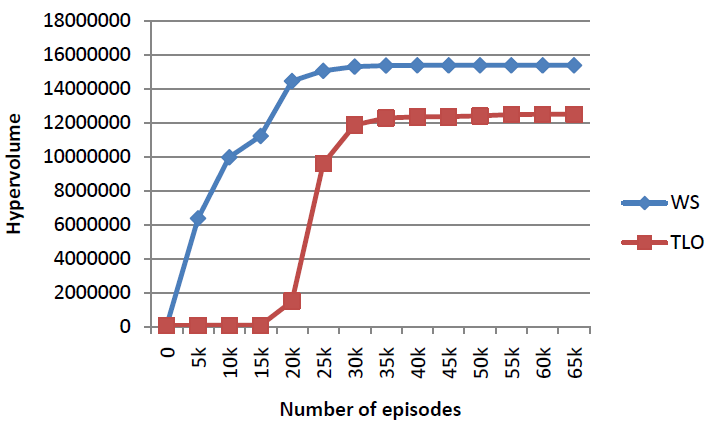
\includegraphics[scale=0.6]{MCResults.png}
\caption{WS vs TLO hypervolume growth on MO-MountainCar problem. Starting position is always fixed and is -0.5. Reference point is (-300;-300;-300). Epsilon is 0.0, alpha is 0.9, gamma is 1.0.}
\label{fig:ws-tlo-mc-results}
\end{figure}

\section{Conclusion.}
Three different problems were presented. Deep Sea Treasure and MO-PuddleWorld has similar reward structure. In that one of the objectives is extrinsic and the other one is intrinsic. Meanwhile the MO-MountainCar has all of its objectives being intrinsic.

Deep Sea Treasure has a number of concavities in Pareto front. The TLO algorithm clearly benefited from its ability to locate those concavities. The WS algorithm doesn’t have this ability and this leads to a situation where the WS algorithm was dominated by the TLO algorithm. The MO-PuddleWorld’s reward structure is similar to the one of Deep Sea Treasure but this doesn’t lead to similar dominance. This can be explained by the nature of the MO-PuddleWorld problem. The MO-PuddleWorld’s Pareto front from any starting position has concavities, but the number of those concavities is not comparable to Deep Sea Treasure and for some starting positions there are no concavities at all. This lead to a situation where the TLO algorithm was not able to benefit from its main strength and showed similar results as the WS algorithm. The MO-MountainCar benchmark highlighted the dominance of the WS algorithm over the TLO in problems with intrinsic rewards.

In summary this chapter demonstrates the importance of empirical studies on benchmark problems with known characteristics in establishing the conditions under which different MORL algorithms will work effectively. Clearly the TLO algorithm can only be used reliably on problems with no more than one intrinsic reward. However where the reward structure of an environment does meet this criteria, TLO is likely to outperform WS due to its capacity to discover policies which lie in concave regions of the Pareto front which cannot be found by the WS algorithm.


%\chapter{Simultaneous Learning of a Multiple Number of Policies.}

Intoductory text.

\section{Stationary Policy.}

Describe a mechanic of fixing one policy as active.

\subsection{Empirical results.}

Show the results of a simultaneous evaluation of more then one policy.

\subsection{Limitations.}

Describe how using only one policy as active may result in insufficient information about an environment state transition dynamics, which in turn may result in incorrect value functions.

\section{Non-stationary Policy.}

Describe how switching active policy helps to alleviate the shortcomings of using stationary policy.

\subsection{Switching states.}

Describe the need to have a state in which the decision about which base policy to use as active.

\subsection{W-Steering}

Descirbe algorithms details.

\subsection{W-Steering Empirical Results}

Show that W-Steering can deliver results in some of the cases but also has shortcomings in other cases.

\subsection{W-Steering Shortcomings.}

Speculate on the reasons why W-Steering may not deliver proper results. Describe the idea of switching states and how having of not having knowledge about them affects 

P

%\chapter{Non-stationary policy evaluation without knowledge of a 'Switching state'}

\section{Introduction}

Describe the need to have an algorithm that can operate under conditions of not having a well-defined 'switching states'. Make a connection with previous chapter.

\section{Q-Steering.}

Introduce Q-Steering algorithm. Describe how it can operate without knowledge of 'switching state'.

\section{Q-Steering Empirical Results.}

Show the results of the benchmarks and demonstrate that Q-Steering is in fact able to deliver its promises.






%\chapter{Case Study.}

Descirbe SCIRO Smart Energy experiment.





\cleardoublepage%was having a problem with page number in contents, this fixes it but creates a problem in hyperref
\phantomsection% this fixes hyperref
\addcontentsline{toc}{chapter}{Conclusions}
\include{conclusions}



\bibliographystyle{ubthesis}
%\bibliographystyle{apacite}
%\bibliographystyle{plainnat}

\cleardoublepage%was having a problem with page number in contents, this fixes it but creates a problem in hyperref
\phantomsection% this fixes hyperref

\addcontentsline{toc}{chapter}{\textbf{References}}
\bibliography{phdreferences}


%\nocite{*}

\appendix % all \chapter{..} commands after this will generate appendices

%\chapter{Conclusion}
%\label{app:example}
%An appendix before the backmatter gets an automatically generated letter by
%which it can be referred to. This is Appendix~\ref{app:example}.

%\chapter{Simulation Source Code}
%You may want to investigate the \texttt{lgrind} program and package if you
%wish to include source code in your thesis

%%%%%%%%%%%%%%%%%%%%%%%%%%%%%%%%%%%%%%%%%%%%%%%%%%%%%%%%%%%%%%%%%%%%%%%%%%%%%%
%%
%% Back matter
%%

\backmatter
%\section*{Conclusion}         % start the thesis back matter
%\begin{thesisauthorvita}
%\begin{spacing}{1}
%Publications arising from this thesis include:
%\begin{description}
%\item[Author, A.\ and Bloggs, J.\ (2002),]
%A really catchy title. In \emph{The 31st International Conference
%on Non-specific Computing.} Capital City, Country.
%\item[Bloggs, J.\ and Author , A. (2002),]
%A very much longer and significantly less catchy title. in \emph {Workshop on
%A Research Area}. Springfield, USA.
%\end{description}
%\end{spacing}
%\end{thesisauthorvita}





%\chapter{Last Thing} % Appendices after the \backmatter command do not
                        % get a letter
%This sort of appendix has no letter.




\end{document}
